\documentclass{article} 
\usepackage{iclr2027_conference,times}
%%%%% NEW MATH DEFINITIONS %%%%%

\usepackage{amsmath,amsfonts,bm}

% Mark sections of captions for referring to divisions of figures
\newcommand{\figleft}{{\em (Left)}}
\newcommand{\figcenter}{{\em (Center)}}
\newcommand{\figright}{{\em (Right)}}
\newcommand{\figtop}{{\em (Top)}}
\newcommand{\figbottom}{{\em (Bottom)}}
\newcommand{\captiona}{{\em (a)}}
\newcommand{\captionb}{{\em (b)}}
\newcommand{\captionc}{{\em (c)}}
\newcommand{\captiond}{{\em (d)}}

% Highlight a newly defined term
\newcommand{\newterm}[1]{{\bf #1}}


% Figure reference, lower-case.
\def\figref#1{figure~\ref{#1}}
% Figure reference, capital. For start of sentence
\def\Figref#1{Figure~\ref{#1}}
\def\twofigref#1#2{figures \ref{#1} and \ref{#2}}
\def\quadfigref#1#2#3#4{figures \ref{#1}, \ref{#2}, \ref{#3} and \ref{#4}}
% Section reference, lower-case.
\def\secref#1{section~\ref{#1}}
% Section reference, capital.
\def\Secref#1{Section~\ref{#1}}
% Reference to two sections.
\def\twosecrefs#1#2{sections \ref{#1} and \ref{#2}}
% Reference to three sections.
\def\secrefs#1#2#3{sections \ref{#1}, \ref{#2} and \ref{#3}}
% Reference to an equation, lower-case.
\def\eqref#1{equation~\ref{#1}}
% Reference to an equation, upper case
\def\Eqref#1{Equation~\ref{#1}}
% A raw reference to an equation---avoid using if possible
\def\plaineqref#1{\ref{#1}}
% Reference to a chapter, lower-case.
\def\chapref#1{chapter~\ref{#1}}
% Reference to an equation, upper case.
\def\Chapref#1{Chapter~\ref{#1}}
% Reference to a range of chapters
\def\rangechapref#1#2{chapters\ref{#1}--\ref{#2}}
% Reference to an algorithm, lower-case.
\def\algref#1{algorithm~\ref{#1}}
% Reference to an algorithm, upper case.
\def\Algref#1{Algorithm~\ref{#1}}
\def\twoalgref#1#2{algorithms \ref{#1} and \ref{#2}}
\def\Twoalgref#1#2{Algorithms \ref{#1} and \ref{#2}}
% Reference to a part, lower case
\def\partref#1{part~\ref{#1}}
% Reference to a part, upper case
\def\Partref#1{Part~\ref{#1}}
\def\twopartref#1#2{parts \ref{#1} and \ref{#2}}

\def\ceil#1{\lceil #1 \rceil}
\def\floor#1{\lfloor #1 \rfloor}
\def\1{\bm{1}}
\newcommand{\train}{\mathcal{D}}
\newcommand{\valid}{\mathcal{D_{\mathrm{valid}}}}
\newcommand{\test}{\mathcal{D_{\mathrm{test}}}}

\def\eps{{\epsilon}}


% Random variables
\def\reta{{\textnormal{$\eta$}}}
\def\ra{{\textnormal{a}}}
\def\rb{{\textnormal{b}}}
\def\rc{{\textnormal{c}}}
\def\rd{{\textnormal{d}}}
\def\re{{\textnormal{e}}}
\def\rf{{\textnormal{f}}}
\def\rg{{\textnormal{g}}}
\def\rh{{\textnormal{h}}}
\def\ri{{\textnormal{i}}}
\def\rj{{\textnormal{j}}}
\def\rk{{\textnormal{k}}}
\def\rl{{\textnormal{l}}}
% rm is already a command, just don't name any random variables m
\def\rn{{\textnormal{n}}}
\def\ro{{\textnormal{o}}}
\def\rp{{\textnormal{p}}}
\def\rq{{\textnormal{q}}}
\def\rr{{\textnormal{r}}}
\def\rs{{\textnormal{s}}}
\def\rt{{\textnormal{t}}}
\def\ru{{\textnormal{u}}}
\def\rv{{\textnormal{v}}}
\def\rw{{\textnormal{w}}}
\def\rx{{\textnormal{x}}}
\def\ry{{\textnormal{y}}}
\def\rz{{\textnormal{z}}}

% Random vectors
\def\rvepsilon{{\mathbf{\epsilon}}}
\def\rvtheta{{\mathbf{\theta}}}
\def\rva{{\mathbf{a}}}
\def\rvb{{\mathbf{b}}}
\def\rvc{{\mathbf{c}}}
\def\rvd{{\mathbf{d}}}
\def\rve{{\mathbf{e}}}
\def\rvf{{\mathbf{f}}}
\def\rvg{{\mathbf{g}}}
\def\rvh{{\mathbf{h}}}
\def\rvu{{\mathbf{i}}}
\def\rvj{{\mathbf{j}}}
\def\rvk{{\mathbf{k}}}
\def\rvl{{\mathbf{l}}}
\def\rvm{{\mathbf{m}}}
\def\rvn{{\mathbf{n}}}
\def\rvo{{\mathbf{o}}}
\def\rvp{{\mathbf{p}}}
\def\rvq{{\mathbf{q}}}
\def\rvr{{\mathbf{r}}}
\def\rvs{{\mathbf{s}}}
\def\rvt{{\mathbf{t}}}
\def\rvu{{\mathbf{u}}}
\def\rvv{{\mathbf{v}}}
\def\rvw{{\mathbf{w}}}
\def\rvx{{\mathbf{x}}}
\def\rvy{{\mathbf{y}}}
\def\rvz{{\mathbf{z}}}

% Elements of random vectors
\def\erva{{\textnormal{a}}}
\def\ervb{{\textnormal{b}}}
\def\ervc{{\textnormal{c}}}
\def\ervd{{\textnormal{d}}}
\def\erve{{\textnormal{e}}}
\def\ervf{{\textnormal{f}}}
\def\ervg{{\textnormal{g}}}
\def\ervh{{\textnormal{h}}}
\def\ervi{{\textnormal{i}}}
\def\ervj{{\textnormal{j}}}
\def\ervk{{\textnormal{k}}}
\def\ervl{{\textnormal{l}}}
\def\ervm{{\textnormal{m}}}
\def\ervn{{\textnormal{n}}}
\def\ervo{{\textnormal{o}}}
\def\ervp{{\textnormal{p}}}
\def\ervq{{\textnormal{q}}}
\def\ervr{{\textnormal{r}}}
\def\ervs{{\textnormal{s}}}
\def\ervt{{\textnormal{t}}}
\def\ervu{{\textnormal{u}}}
\def\ervv{{\textnormal{v}}}
\def\ervw{{\textnormal{w}}}
\def\ervx{{\textnormal{x}}}
\def\ervy{{\textnormal{y}}}
\def\ervz{{\textnormal{z}}}

% Random matrices
\def\rmA{{\mathbf{A}}}
\def\rmB{{\mathbf{B}}}
\def\rmC{{\mathbf{C}}}
\def\rmD{{\mathbf{D}}}
\def\rmE{{\mathbf{E}}}
\def\rmF{{\mathbf{F}}}
\def\rmG{{\mathbf{G}}}
\def\rmH{{\mathbf{H}}}
\def\rmI{{\mathbf{I}}}
\def\rmJ{{\mathbf{J}}}
\def\rmK{{\mathbf{K}}}
\def\rmL{{\mathbf{L}}}
\def\rmM{{\mathbf{M}}}
\def\rmN{{\mathbf{N}}}
\def\rmO{{\mathbf{O}}}
\def\rmP{{\mathbf{P}}}
\def\rmQ{{\mathbf{Q}}}
\def\rmR{{\mathbf{R}}}
\def\rmS{{\mathbf{S}}}
\def\rmT{{\mathbf{T}}}
\def\rmU{{\mathbf{U}}}
\def\rmV{{\mathbf{V}}}
\def\rmW{{\mathbf{W}}}
\def\rmX{{\mathbf{X}}}
\def\rmY{{\mathbf{Y}}}
\def\rmZ{{\mathbf{Z}}}

% Elements of random matrices
\def\ermA{{\textnormal{A}}}
\def\ermB{{\textnormal{B}}}
\def\ermC{{\textnormal{C}}}
\def\ermD{{\textnormal{D}}}
\def\ermE{{\textnormal{E}}}
\def\ermF{{\textnormal{F}}}
\def\ermG{{\textnormal{G}}}
\def\ermH{{\textnormal{H}}}
\def\ermI{{\textnormal{I}}}
\def\ermJ{{\textnormal{J}}}
\def\ermK{{\textnormal{K}}}
\def\ermL{{\textnormal{L}}}
\def\ermM{{\textnormal{M}}}
\def\ermN{{\textnormal{N}}}
\def\ermO{{\textnormal{O}}}
\def\ermP{{\textnormal{P}}}
\def\ermQ{{\textnormal{Q}}}
\def\ermR{{\textnormal{R}}}
\def\ermS{{\textnormal{S}}}
\def\ermT{{\textnormal{T}}}
\def\ermU{{\textnormal{U}}}
\def\ermV{{\textnormal{V}}}
\def\ermW{{\textnormal{W}}}
\def\ermX{{\textnormal{X}}}
\def\ermY{{\textnormal{Y}}}
\def\ermZ{{\textnormal{Z}}}

% Vectors
\def\vzero{{\bm{0}}}
\def\vone{{\bm{1}}}
\def\vmu{{\bm{\mu}}}
\def\vtheta{{\bm{\theta}}}
\def\va{{\bm{a}}}
\def\vb{{\bm{b}}}
\def\vc{{\bm{c}}}
\def\vd{{\bm{d}}}
\def\ve{{\bm{e}}}
\def\vf{{\bm{f}}}
\def\vg{{\bm{g}}}
\def\vh{{\bm{h}}}
\def\vi{{\bm{i}}}
\def\vj{{\bm{j}}}
\def\vk{{\bm{k}}}
\def\vl{{\bm{l}}}
\def\vm{{\bm{m}}}
\def\vn{{\bm{n}}}
\def\vo{{\bm{o}}}
\def\vp{{\bm{p}}}
\def\vq{{\bm{q}}}
\def\vr{{\bm{r}}}
\def\vs{{\bm{s}}}
\def\vt{{\bm{t}}}
\def\vu{{\bm{u}}}
\def\vv{{\bm{v}}}
\def\vw{{\bm{w}}}
\def\vx{{\bm{x}}}
\def\vy{{\bm{y}}}
\def\vz{{\bm{z}}}

% Elements of vectors
\def\evalpha{{\alpha}}
\def\evbeta{{\beta}}
\def\evepsilon{{\epsilon}}
\def\evlambda{{\lambda}}
\def\evomega{{\omega}}
\def\evmu{{\mu}}
\def\evpsi{{\psi}}
\def\evsigma{{\sigma}}
\def\evtheta{{\theta}}
\def\eva{{a}}
\def\evb{{b}}
\def\evc{{c}}
\def\evd{{d}}
\def\eve{{e}}
\def\evf{{f}}
\def\evg{{g}}
\def\evh{{h}}
\def\evi{{i}}
\def\evj{{j}}
\def\evk{{k}}
\def\evl{{l}}
\def\evm{{m}}
\def\evn{{n}}
\def\evo{{o}}
\def\evp{{p}}
\def\evq{{q}}
\def\evr{{r}}
\def\evs{{s}}
\def\evt{{t}}
\def\evu{{u}}
\def\evv{{v}}
\def\evw{{w}}
\def\evx{{x}}
\def\evy{{y}}
\def\evz{{z}}

% Matrix
\def\mA{{\bm{A}}}
\def\mB{{\bm{B}}}
\def\mC{{\bm{C}}}
\def\mD{{\bm{D}}}
\def\mE{{\bm{E}}}
\def\mF{{\bm{F}}}
\def\mG{{\bm{G}}}
\def\mH{{\bm{H}}}
\def\mI{{\bm{I}}}
\def\mJ{{\bm{J}}}
\def\mK{{\bm{K}}}
\def\mL{{\bm{L}}}
\def\mM{{\bm{M}}}
\def\mN{{\bm{N}}}
\def\mO{{\bm{O}}}
\def\mP{{\bm{P}}}
\def\mQ{{\bm{Q}}}
\def\mR{{\bm{R}}}
\def\mS{{\bm{S}}}
\def\mT{{\bm{T}}}
\def\mU{{\bm{U}}}
\def\mV{{\bm{V}}}
\def\mW{{\bm{W}}}
\def\mX{{\bm{X}}}
\def\mY{{\bm{Y}}}
\def\mZ{{\bm{Z}}}
\def\mBeta{{\bm{\beta}}}
\def\mPhi{{\bm{\Phi}}}
\def\mLambda{{\bm{\Lambda}}}
\def\mSigma{{\bm{\Sigma}}}

% Tensor
\DeclareMathAlphabet{\mathsfit}{\encodingdefault}{\sfdefault}{m}{sl}
\SetMathAlphabet{\mathsfit}{bold}{\encodingdefault}{\sfdefault}{bx}{n}
\newcommand{\tens}[1]{\bm{\mathsfit{#1}}}
\def\tA{{\tens{A}}}
\def\tB{{\tens{B}}}
\def\tC{{\tens{C}}}
\def\tD{{\tens{D}}}
\def\tE{{\tens{E}}}
\def\tF{{\tens{F}}}
\def\tG{{\tens{G}}}
\def\tH{{\tens{H}}}
\def\tI{{\tens{I}}}
\def\tJ{{\tens{J}}}
\def\tK{{\tens{K}}}
\def\tL{{\tens{L}}}
\def\tM{{\tens{M}}}
\def\tN{{\tens{N}}}
\def\tO{{\tens{O}}}
\def\tP{{\tens{P}}}
\def\tQ{{\tens{Q}}}
\def\tR{{\tens{R}}}
\def\tS{{\tens{S}}}
\def\tT{{\tens{T}}}
\def\tU{{\tens{U}}}
\def\tV{{\tens{V}}}
\def\tW{{\tens{W}}}
\def\tX{{\tens{X}}}
\def\tY{{\tens{Y}}}
\def\tZ{{\tens{Z}}}


% Graph
\def\gA{{\mathcal{A}}}
\def\gB{{\mathcal{B}}}
\def\gC{{\mathcal{C}}}
\def\gD{{\mathcal{D}}}
\def\gE{{\mathcal{E}}}
\def\gF{{\mathcal{F}}}
\def\gG{{\mathcal{G}}}
\def\gH{{\mathcal{H}}}
\def\gI{{\mathcal{I}}}
\def\gJ{{\mathcal{J}}}
\def\gK{{\mathcal{K}}}
\def\gL{{\mathcal{L}}}
\def\gM{{\mathcal{M}}}
\def\gN{{\mathcal{N}}}
\def\gO{{\mathcal{O}}}
\def\gP{{\mathcal{P}}}
\def\gQ{{\mathcal{Q}}}
\def\gR{{\mathcal{R}}}
\def\gS{{\mathcal{S}}}
\def\gT{{\mathcal{T}}}
\def\gU{{\mathcal{U}}}
\def\gV{{\mathcal{V}}}
\def\gW{{\mathcal{W}}}
\def\gX{{\mathcal{X}}}
\def\gY{{\mathcal{Y}}}
\def\gZ{{\mathcal{Z}}}

% Sets
\def\sA{{\mathbb{A}}}
\def\sB{{\mathbb{B}}}
\def\sC{{\mathbb{C}}}
\def\sD{{\mathbb{D}}}
% Don't use a set called E, because this would be the same as our symbol
% for expectation.
\def\sF{{\mathbb{F}}}
\def\sG{{\mathbb{G}}}
\def\sH{{\mathbb{H}}}
\def\sI{{\mathbb{I}}}
\def\sJ{{\mathbb{J}}}
\def\sK{{\mathbb{K}}}
\def\sL{{\mathbb{L}}}
\def\sM{{\mathbb{M}}}
\def\sN{{\mathbb{N}}}
\def\sO{{\mathbb{O}}}
\def\sP{{\mathbb{P}}}
\def\sQ{{\mathbb{Q}}}
\def\sR{{\mathbb{R}}}
\def\sS{{\mathbb{S}}}
\def\sT{{\mathbb{T}}}
\def\sU{{\mathbb{U}}}
\def\sV{{\mathbb{V}}}
\def\sW{{\mathbb{W}}}
\def\sX{{\mathbb{X}}}
\def\sY{{\mathbb{Y}}}
\def\sZ{{\mathbb{Z}}}

% Entries of a matrix
\def\emLambda{{\Lambda}}
\def\emA{{A}}
\def\emB{{B}}
\def\emC{{C}}
\def\emD{{D}}
\def\emE{{E}}
\def\emF{{F}}
\def\emG{{G}}
\def\emH{{H}}
\def\emI{{I}}
\def\emJ{{J}}
\def\emK{{K}}
\def\emL{{L}}
\def\emM{{M}}
\def\emN{{N}}
\def\emO{{O}}
\def\emP{{P}}
\def\emQ{{Q}}
\def\emR{{R}}
\def\emS{{S}}
\def\emT{{T}}
\def\emU{{U}}
\def\emV{{V}}
\def\emW{{W}}
\def\emX{{X}}
\def\emY{{Y}}
\def\emZ{{Z}}
\def\emSigma{{\Sigma}}

% entries of a tensor
% Same font as tensor, without \bm wrapper
\newcommand{\etens}[1]{\mathsfit{#1}}
\def\etLambda{{\etens{\Lambda}}}
\def\etA{{\etens{A}}}
\def\etB{{\etens{B}}}
\def\etC{{\etens{C}}}
\def\etD{{\etens{D}}}
\def\etE{{\etens{E}}}
\def\etF{{\etens{F}}}
\def\etG{{\etens{G}}}
\def\etH{{\etens{H}}}
\def\etI{{\etens{I}}}
\def\etJ{{\etens{J}}}
\def\etK{{\etens{K}}}
\def\etL{{\etens{L}}}
\def\etM{{\etens{M}}}
\def\etN{{\etens{N}}}
\def\etO{{\etens{O}}}
\def\etP{{\etens{P}}}
\def\etQ{{\etens{Q}}}
\def\etR{{\etens{R}}}
\def\etS{{\etens{S}}}
\def\etT{{\etens{T}}}
\def\etU{{\etens{U}}}
\def\etV{{\etens{V}}}
\def\etW{{\etens{W}}}
\def\etX{{\etens{X}}}
\def\etY{{\etens{Y}}}
\def\etZ{{\etens{Z}}}

% The true underlying data generating distribution
\newcommand{\pdata}{p_{\rm{data}}}
% The empirical distribution defined by the training set
\newcommand{\ptrain}{\hat{p}_{\rm{data}}}
\newcommand{\Ptrain}{\hat{P}_{\rm{data}}}
% The model distribution
\newcommand{\pmodel}{p_{\rm{model}}}
\newcommand{\Pmodel}{P_{\rm{model}}}
\newcommand{\ptildemodel}{\tilde{p}_{\rm{model}}}
% Stochastic autoencoder distributions
\newcommand{\pencode}{p_{\rm{encoder}}}
\newcommand{\pdecode}{p_{\rm{decoder}}}
\newcommand{\precons}{p_{\rm{reconstruct}}}

\newcommand{\laplace}{\mathrm{Laplace}} % Laplace distribution

\newcommand{\E}{\mathbb{E}}
\newcommand{\Ls}{\mathcal{L}}
\newcommand{\R}{\mathbb{R}}
\newcommand{\emp}{\tilde{p}}
\newcommand{\lr}{\alpha}
\newcommand{\reg}{\lambda}
\newcommand{\rect}{\mathrm{rectifier}}
\newcommand{\softmax}{\mathrm{softmax}}
\newcommand{\sigmoid}{\sigma}
\newcommand{\softplus}{\zeta}
\newcommand{\KL}{D_{\mathrm{KL}}}
\newcommand{\Var}{\mathrm{Var}}
\newcommand{\standarderror}{\mathrm{SE}}
\newcommand{\Cov}{\mathrm{Cov}}
% Wolfram Mathworld says $L^2$ is for function spaces and $\ell^2$ is for vectors
% But then they seem to use $L^2$ for vectors throughout the site, and so does
% wikipedia.
\newcommand{\normlzero}{L^0}
\newcommand{\normlone}{L^1}
\newcommand{\normltwo}{L^2}
\newcommand{\normlp}{L^p}
\newcommand{\normmax}{L^\infty}

\newcommand{\parents}{Pa} % See usage in notation.tex. Chosen to match Daphne's book.

\DeclareMathOperator*{\argmax}{arg\,max}
\DeclareMathOperator*{\argmin}{arg\,min}

\DeclareMathOperator{\sign}{sign}
\DeclareMathOperator{\Tr}{Tr}
\let\ab\allowbreak


\usepackage{hyperref}
\usepackage{url}
\usepackage{amsmath}
\usepackage{booktabs}
\usepackage{graphicx}
\usepackage{xcolor}

% ---------------------------------------------------------------------
% Revision colours (post-discussion revision). One switch: REVISED_CLEAN.tex
% defines \revclean before \input-ing this file, which prints everything in black.
% RL5B = blue, Caus = teal, dypE = purple, two or more reviewers = orange.
% ---------------------------------------------------------------------
\newif\ifrevmarked \revmarkedtrue
\ifdefined\revclean \revmarkedfalse \fi
\definecolor{RevA}{RGB}{0,72,190}       % RL5B only: blue
\definecolor{RevB}{RGB}{0,115,115}      % Caus only: teal
\definecolor{RevC}{RGB}{105,45,160}     % dypE only: purple
\definecolor{RevShared}{RGB}{190,85,0}  % two or more reviewers: orange
\DeclareRobustCommand{\revA}[1]{\ifrevmarked{\color{RevA}#1}\else{#1}\fi}
\DeclareRobustCommand{\revB}[1]{\ifrevmarked{\color{RevB}#1}\else{#1}\fi}
\DeclareRobustCommand{\revC}[1]{\ifrevmarked{\color{RevC}#1}\else{#1}\fi}
\DeclareRobustCommand{\revShared}[1]{\ifrevmarked{\color{RevShared}#1}\else{#1}\fi}
% for multi-paragraph spans and \input files
\newenvironment{revblock}[1]{\ifrevmarked\color{#1}\fi}{}
% for whole floats: place right after \begin{table}
\newcommand{\revfloatcolor}[1]{\ifrevmarked\color{#1}\fi}


\newcommand{\atemp}{\tau}
% The dose-response verdict is the pre-registered decision sentence, generated from the committed result
% (cdr_result.tex). The confirmatory-equivalence numbers are written out in Section 3.1 and Table 3 with all
% three arms' seed counts (16/15/15), so the generated EQ sentence is no longer used.
\newcommand{\cdrverdict}{\textbf{[dose-response result pending]}}
\newcommand{\cdrshort}{\textbf{[one-sentence dose-response result pending]}}
% Generated by analysis/make_cdr_sentences.py from RESULT_TABLES/EXP02_SINet_summary.json -- do not edit by hand.
\renewcommand{\cdrverdict}{It did not support a downstream effect of concentration. On SINet the twice-as-concentrated level differs from the dispersed references by $+0.0021$ Boundary-IoU and the committed shape by $-0.0005$, against a bar of $0.0193$ ($0.11\times$ and $0.03\times$), and no secondary measure on COD10K-test, $S_\alpha$ included, clears its bar. We therefore restrict the concentration claim to the training-set distribution: concentration explains why targeted training sets look different, not a change in accuracy.}
\renewcommand{\cdrshort}{A pre-registered dose-response experiment found no downstream effect of concentration on accuracy, so the concentration claim is restricted to the training sets.}
  % dose-response result, filled 2026-11-16 from the pre-registered sentence

\title{Concentration, Not Uncertainty: Why Targeted Synthetic Data Doesn't Help Camouflaged Object Detection}

% Authors must not appear in the submitted version. They should be hidden
% as long as the \iclrfinalcopy macro remains commented out below.
% Non-anonymous submissions will be rejected without review.

\author{Anonymous Authors \\
Anonymous Institution \\
\texttt{anonymous@example.com}
}

%\iclrfinalcopy % Uncomment for camera-ready version, but NOT for submission.
\begin{document}

\maketitle

% =====================================================================
% ABSTRACT -- gate 9 (last).  <= 160 words, <= 8 numbers, written to cap.
% =====================================================================
\begin{abstract}
%Camouflaged object detection needs pixel-accurate masks that are slow and costly to draw, so
%synthetic training images are a standard remedy. That raises a question nobody has answered: under a
%fixed budget, which images should you generate? The obvious answer is to let the model choose, and
%we built that loop ; cluster the unlabelled real images the model will face, find the clusters it
%is least sure about, aim the generation there, retrain, repeat.
%
%No advantage survives measurement. Across $103$ trained runs, targeting does not beat random
%allocation, and five independent controls each close a different reason that null might be an
%artifact. The reason is itself a positive finding: a targeted training set
%\emph{is} measurably different from a random one, but the difference comes from concentrating the
%budget rather than aiming it ; every concentrating rule we tested reproduces it, and on boundary
%accuracy so does one that reverses the uncertainty signal outright. Separately, $50$ of
%CHAMELEON's $76$ images are copies of training data, while the standard check reports $0$ overlap.

Camouflaged object detection requires pixel-accurate masks, but obtaining such annotations is slow and costly, making synthetic training images an attractive alternative. Under a fixed generation budget, however, it remains unclear which real-image regions to target for synthetic data generation. We study an uncertainty-guided \revShared{allocation} strategy that clusters the unlabelled real images, identifies clusters on which the model is least certain, allocates \revShared{a fixed pool of synthetic images} toward those clusters, and retrains the model. \revShared{Within the pipeline we test, uncertainty-guided allocation shows no detectable benefit over random allocation across 103 training runs, and a pre-registered confirmatory campaign establishes equivalence within $\pm0.005$ $S_\alpha$ on the primary comparison (90\% interval $-0.0027$ to $+0.0039$). Same-shape controls show that the direction of the uncertainty signal adds nothing detectable.} Targeted training sets are nonetheless measurably different from random ones, \revB{and how the selector matches images to clusters and how unevenly it spreads the budget explain that difference, not where the budget is aimed}; \revShared{a pre-registered dose-response test found no effect of concentration on accuracy.} Separately, we find substantial data contamination in CHAMELEON, with \revC{at least} 50 of its 76 images duplicated from training data despite the standard overlap check reporting zero overlap. \revShared{These conclusions are bounded to the setting tested: allocation over a fixed, offline pool of LAKE-RED renders that re-use 4,447 foregrounds with new backgrounds, the S2R-COD two-round protocol, $k = 75$ clusters of frozen self-supervised features, SINet and SINet-v2, and a budget of 1,000 images.}
\end{abstract}

% =====================================================================
\section{Introduction}
\label{sec:intro}
Camouflaged object detection is a task aimed at generating an accurate pixel-level outline of an animal that evolved to blend into its surroundings. Its training masks are unusually expensive for exactly that reason: an annotator must
decide where a boundary lies when the point of the object is to conceal its boundary. One standard response to the resulting scarcity is to manufacture more data. A generator takes a real
cutout object and paints a fresh background around it, producing a new labeled pair at no
annotation cost.


Generation is not free either, and every generated image has to be trained on. So if you generate
a thousand of them, which thousand? Our answer is to let the model guide its own data generation: After initial training, we evaluate the model on unlabelled real images, identify the regions where highest uncertainty is observed, and target our synthetic data generation toward those regions. Every ingredient of that loop is standard
(Section~\ref{sec:related}); the composition is ours, and we failed to make it function.


A targeted training set really is measurably different from a random one of the same size: a classifier, shown images from each, learns to tell which set an image came from even images it never saw. But it is picking up \revB{how the set was filled}, not aim. Targeting piles the budget onto a few clusters, and any rule that piles it the same way works just as well: point the same lopsided budget at the wrong clusters and the classifier still wins. \revB{Only a random draw defeats it; even a perfectly even quota, filled by the same matching to cluster centres, does not.} What looked like an effect of targeting on the training set was an effect of \revB{matching and} concentrating it; the
comparison that settles this is not a random set, but one with the same lopsided shape
aimed at nothing in particular. \revShared{Whether concentration also changes trained accuracy is a separate question, and we
test it directly rather than infer it from the training sets.}


In terms of trained accuracy, targeting shows \revShared{no detectable advantage} over random allocation. That null is
bounded rather than absolute: \revShared{at eight seeds it excludes an advantage the size of the published method's own gain
but not smaller ones, and a pre-registered confirmatory campaign then establishes equivalence within $\pm0.005$
$S_\alpha$ on the primary comparison;} a positive control confirms that the measurement
detects a real effect.
\revB{Re-ranking the same allocation by each cluster's test-set error produces no detectable change, and neither do
oracle allocations of three other shapes.} Extending training to accommodate extra images without reducing steps on real data shows no improvement. Separately, we expose a major flaw in the standard CHAMELEON test set, where \revC{at least} 50 of its 76 images are direct copies from COD10K and CAMO training sets. Standard duplicate checks fail to flag these because they were re-saved in different formats, eliminating byte-level matches. The main contributions of this paper are:

\begin{itemize}
\item \textit{A control} that separates aiming a generation budget from merely concentrating it. Because a steered selection differs from random in two ways at once where it points and how unevenly it is spread a random baseline conflates them. Ours fixes the shape and scrambles only the signal; our own method does not survive it.
\item \textit{A bounded null on the direction}: \revShared{no detectable advantage, with the sizes of effect that are and are
not excluded stated, a pre-registered confirmatory test of equivalence,} and five independent controls: a positive control, \revB{an endpoint-error oracle at the committed shape and at three others}, an unpinned
optimization schedule, a same-shape shuffle, and a seed expansion.
\item \textit{Three checks run before any training} and precede any cluster-wise acquisition
policy: whether the target data clusters at all, what the funded clusters are made of, and how much of the endpoint's error sits between clusters rather than within them.
\item \textit{CHAMELEON is \revC{at least} $50$ of $76$ images ($65.8\%$) training data} for models trained on
COD10K, while exact hashing reports $0$ overlap; we release a re-encode-tolerant detector, the
confirmed pair list and a clean evaluation protocol.
\end{itemize}
\revShared{These conclusions concern the allocation of a fixed, background-varied render pool, not uncertainty-guided generation
in general; Section~\ref{sec:discussion} states the scope exactly.}


% =====================================================================
\subsection{Related Work}
\label{sec:related}
This paper asks whether an \emph{acquisition policy}, a rule for
deciding which synthetic images to generate under a fixed budget can improve a pipeline that is
otherwise held fixed. The task it does that on is camouflaged object detection, which asks for a
pixel-accurate outline of an object whose color and texture are built to defeat exactly that;
\citet{fan2023advances} surveys its architectures, datasets, and evaluation conventions.

A prediction is scored by how well its mask matches the true one. Our primary measure is the \emph{S-measure} $S_\alpha$~\citep{fan2017structure}, which rewards getting an object's \emph{shape} right rather than counting correct pixels, and which runs
from $0$ to $1$ with higher being better. The scale matters for reading everything that follows. Every
camouflaged object detector in this paper scores near $0.70$, so the differences the paper turns on are small fractions
of the range these models actually occupy. Three words then recur. An \textit{arm} is one training
condition; all arms share a base pool of labeled images and differ only in which images are
appended to it. A \textit{seed} is one training run of one arm, repeat runs of the same arm do
not return the same score, and the size of that seed-to-seed spread is what any real difference has
to beat. An \textit{endpoint} is a held-out test set from which a verdict is read. Finally, the
\textit{reference effect} is the improvement this repository reproduced for the published method it
builds on, $0.7030 \rightarrow 0.7172$, or $+0.0142$. That is the size of effect this design had to
be able to resolve, and the yardstick every sensitivity claim in this paper is measured against. The closest are LAKE-RED~\citep{zhao2024lakered}, whose background generation and compositing we use unchanged, and
S2R-COD~\citep{luo2025s2rcod}, whose synthetic-to-real self-training protocol we follow. Relative to
both, the only thing we add is an allocation layer that chooses \emph{which} generated images to
append; the generator, the budget, and the training procedure are left alone. Synthetic-augmentation methods such as DatasetDM~\citep{wu2023datasetdm} address how to construct labeled data at all, which is a different question from how to spend a fixed amount of it. \revA{Unsupervised RISE~\citep{du2025rise} reaches higher absolute accuracy by a different route, pseudo masks on the real target images (Appendix~\ref{app:related}).}

Every part of it is standard. Uncertainty sampling comes from active learning~\citep{settles2009active}, except that our query is answered by a generator rather than by a human annotator; the uncertainty is student-teacher disagreement of the
kind mean-teacher training already minimises~\citep{tarvainen2017mean}; and $k$-means over frozen
self-supervised features~\citep{oquab2024dinov2,radford2021learning} keeps the budget from piling
onto near-duplicates, in the spirit of core-set selection~\citep{sener2018active}. Other
constructions exist: deep ensembles~\citep{lakshminarayanan2017simple},
MC-dropout~\citep{gal2016dropout}, BADGE~\citep{ash2020deep}, and Section~\ref{sec:why} measures
an ensemble and predictive entropy alongside ours, but we propose none. What is contributed here is a controlled test of the composition. 

Three recent systems share the premise that a generation budget should be steered rather than spent uniformly.
GAUDA~\citep{frisch2025gauda} conditions a latent diffusion model on the classes a Bayesian model is
least certain about; DisCL~\citep{liang2025discl} steers image-guidance strength along a curriculum;
SynQuE~\citep{chen2025synque} ranks whole synthetic datasets using only unannotated real data.
\textit{None of the three runs a control that holds the allocation's shape fixed while destroying
the signal inside it}, and that turns out to be the control that decides the question, because a
steered selection differs from a random one in two ways at once, where the budget points, and how
unevenly it is spread. Appendix~\ref{app:related} places these systems side by side and covers
benchmark definitions and generative alternatives. Section~\ref{sec:method} specifies the loop we
built and the arms that separate those two things.

% =====================================================================
\section{Methods}
\label{sec:method}
In this section, we introduce our approach of uncertainty guided generation in the loop. We train a model on a labeled set of images, evaluate on the unlabeled
real images, and find the ones it handles least confidently. Then we ask a generator for
new images resembling those, add them to the training set, and train again. What follows is our
instantiation of that idea, specified exactly, because a null result is only as informative as the
thing it tested.

We train on a \emph{synthetic data source pool} of $4447$ labelled image and mask pairs
and want the model to work on a \emph{target pool} of $4040$ unlabelled real images, with verdicts
read from two held-out endpoints: COD10K-test decides, and NC4K is reported. The target pool is not
one distribution but a mixture of $3040$ COD10K images and $1000$ from CAMO, which matters later
(Section~\ref{sec:why}). Training runs in two rounds: a student trains alongside a teacher that is a slowly updated running
average of its own weights, target images that the two already agree on are appended between rounds with
the teacher's prediction as their label, and round two retrains from scratch on the enlarged pool.
Two properties the phrase ``closed loop'' hides both bound what follows; the round count is a
fixed constant, not a convergence criterion, and the generator renders its pool once, offline, and
is never invoked during training.

A fixed generation budget has to be spent somewhere, and our rule spends it where the model is weakest. \textit{(i) Group the target images}, so that
``weak'' can name a region of the data rather than a single image: $k$-means into $k = 75$ clusters
over L2-normalized self-supervised embeddings, fitted once and never refitted. \textit{(ii) Score
each image for uncertainty.} We need a number, computable without labels, that says how unsure the model is; the natural candidate is how far the student and its own running average disagree, which
is available precisely because the consistency loss is already trying to reduce it:
\begin{equation}
\mathrm{ES}(x) \;=\; a \,\big\| \nabla \sigma(s(x)) - \nabla \sigma(t(x)) \big\|_{1}
\;+\; b \, \mathrm{BCE}\big( \sigma(s(x)),\, \sigma(t(x)) \big),
\label{eq:es}
\end{equation}
with student and teacher logits $s,t$, sigmoid $\sigma$, Sobel gradient magnitude $\nabla$, binary
cross-entropy BCE, and
configured weights $a, b$ in Appendix~\ref{app:method}. What this buys is a score needing no ground
truth, computable on exactly the images the model will be judged on; a cluster's score is the mean
over its members. Its dominant term is the distance between \emph{gradient} magnitudes, which makes it a boundary-focused signal; a fact Section~\ref{sec:concentration} returns to. \textit{(iii) Turn scores into a budget split.} The budget is spread by a softmax over the cluster scores in units of their across-cluster standard deviation, at temperature $\atemp = 1.0$ (Appendix~\ref{app:method}); $\atemp$ sets how sharply the
budget piles onto the worst clusters.
\textit{(iv) Fill each quota} by drawing the foregrounds whose masked cutouts sit closest to the
funded cluster's centroid.

\begin{table}[t]
\caption{Every arm shares one base pool and differs only in what is appended to it. The last two columns are the axes of Figure~\ref{fig:arms}: how concentrated the allocation is, and where it points. The C-family are permutations of a single allocation, so they hold concentration fixed and differ only in direction; the digits in C10 record the allocation temperature,
$\atemp = 1.0$. None of A0, A2 and MT has an allocation to place.}
\label{tab:arms}
\begin{center}
\small
\setlength{\tabcolsep}{4pt}
\begin{tabular}{@{}llll@{}}
\toprule
Arm & What it appends & Concentration & Direction \\
\midrule
A0 & nothing & --- & --- \\
A2 & $1000$ real photographs & --- & --- \\
B & $1000$ renders drawn uniformly at random & dispersed & none \\
C10 & the $1000$ the allocation selects & concentrated & as scored \\
\midrule
CSHUF & C10's quotas, cluster scores permuted & fixed, same shape & destroyed \\
CINV & C10's quotas, their rank reversed & fixed, same shape & reversed \\
CORACLE & C10's quotas, reassigned by true endpoint error & fixed, same shape & true error \\
\midrule
A0FX, BFX, C10FX & A0, B, C10 with the optimisation budget unpinned & as A0, B, C10 & as A0, B, C10 \\
MT & nothing; A0's pool run single-round & --- & --- \\
\bottomrule
\end{tabular}
\end{center}
\end{table}

All arms (Table~\ref{tab:arms}) share the same base pool and differ
only in which $1000$ images are appended to it, so any difference between two of them is
attributable to that choice and nothing else. \textit{A0} appends
nothing. \textit{A2} appends $1000$ real photographs, which separates the effect of a larger pool
from the effect of generated content. \textit{B} appends $1000$ renders drawn uniformly at random,
redrawn per seed. \textit{C10} appends the $1000$ that the allocation above selects. A2, B and C10
all hold $5447$ pairs, and the comparison this paper turns on is C10 against B.

That comparison cannot settle the question on its own, and Figure~\ref{fig:arms} is why: a targeted
allocation differs from a random one along \emph{two} axes at once, it is more concentrated, and
it points somewhere, so a difference between C10 and B is attributable to neither. Three further
arms hold concentration exactly fixed and vary only where the budget points. \textit{CSHUF} permutes
the cluster scores, destroying the signal while preserving the allocation's shape; \textit{CINV}
reverses their rank; \textit{CORACLE} reassigns the quotas based on each cluster's true endpoint error.

\begin{figure}[t]
\begin{center}
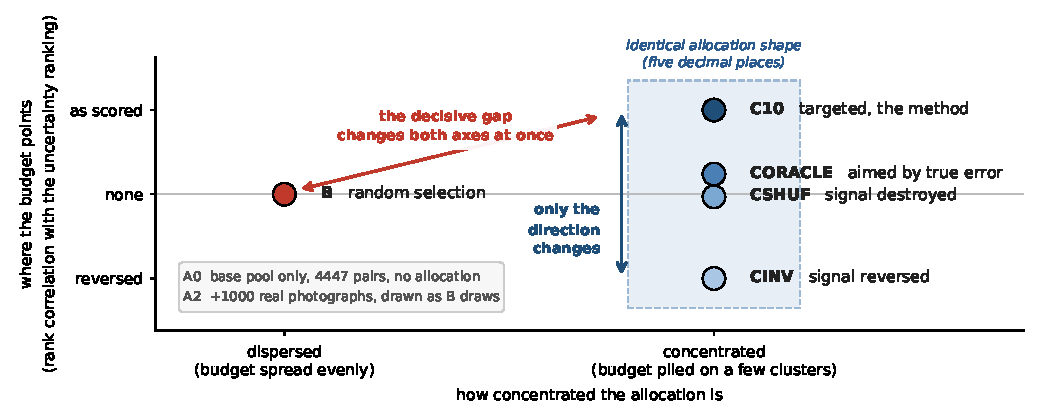
\includegraphics[width=0.95\textwidth]{figs/fig_arms.pdf}
\end{center}
\caption{\textit{What each arm holds fixed and what it varies.} The horizontal axis is how
concentrated an allocation is; the vertical axis is where it points, measured as rank correlation
with the committed uncertainty ranking. Because the C-family are permutations of one allocation,
they reproduce its shape to five decimal places and differ only vertically,  which is what makes
the vertical contrast clean and the diagonal one ambiguous. A0 and A2 append nothing and no
generated content, respectively, so neither has an allocation to place.
\emph{Sources:} \texttt{abc\_pools.json}; \texttt{T2\_RESULTS.md}; \texttt{results.md} \S5.2.}
\label{fig:arms}
\end{figure}

Write $\hat{\sigma}$ for the seed-to-seed wobble, the pooled within-arm standard deviation of $S_\alpha$, taken at the conventional $\alpha = 0.5$. A gap is a \textsc{real effect} only if it exceeds twice that wobble \emph{and} \revA{the seeds agree on
its sign (every seed at three seeds; at least seven of eight in the eight-seed expansion, a threshold fixed before
that campaign ran)}; a smaller gap is \textsc{within noise}; one that clears the bar without agreeing in sign is
\textsc{inconclusive}, and is reported as such rather than resolved by adding seeds. The rule applies
per architecture, and a disagreement between them is reported as a disagreement. We report no
$p$-values at three seeds. Appendix~\ref{app:method} records the rule's provenance, the seeds, and
the gates each campaign passed before launching.

% =====================================================================
\section{Results}
\label{sec:results}
Four analyses follow, each measured independently of the others: whether the targeted allocation
beats a random one on trained accuracy, what makes a targeted set measurably different, regardless of
that null, the mechanism behind the null, and a separate finding about the benchmark used to read all
of the above.

\subsection{Does Targeting Beat Random}
\label{sec:null}
The loop is specified, so the first question is the one it was built to answer. \textit{Aiming the budget by uncertainty \revShared{showed no detectable advantage over} spending it at random.} On the primary endpoint at eight seeds
per arm, the gap between the targeted allocation and a random one is $+0.0024$, about a third of
the spread it would have had to clear, and every one of the sixteen gaps that campaign decides
returns the same verdict.

A null is only as good as the objections it survives, so the rest of this section is those
objections and what each one was answered with. Table~\ref{tab:trained} is the whole trained record: four campaigns that return nothing, and one that returns something, which is how we know the four
nulls mean anything at all.

\begin{table}[t]
\caption{Trained comparison on the primary architecture and endpoint. A gap must
exceed its own campaign's bar \emph{and} agree in sign across seeds to count. Four campaigns attack
the decisive gap from different directions and none of them moves it; the positive control, which
compares against a method we expected to be clearly worse, clears its bar more than threefold.
\revB{ORS (oracle allocations of other shapes) was run after review and reads endpoint labels to choose training data (Appendix~\ref{app:shapeoracle}).}
Per-cell tables for both architectures and both endpoints are in Appendix~\ref{app:diag}.
\emph{Sources:} \texttt{abc\_verdict.json} and its \texttt{or/}, \texttt{fx/}, \texttt{se/}
variants; \texttt{pc\_verdict.json}.}
\label{tab:trained}
\begin{center}
\small
\setlength{\tabcolsep}{2.5pt}
\begin{tabular}{@{}llcccccl@{}}
\toprule
& What it tests & $n$ & Gap & $\Delta$ & $2\hat{\sigma}$ & $\times$\,bar & Verdict \\
\midrule
ABC & targeting vs.\ random, as committed & $3$ & C10$-$B & $+0.0050$ & $0.0179$ & $0.28$ & \textsc{within noise} \\
SE & the same gap at eight seeds & $8$ & C10$-$B & $+0.0024$ & $0.0069$ & $0.34$ & \textsc{within noise} \\
OR & a perfect score in place of ours & $3$ & CORACLE$-$B & $+0.0008$ & $0.0061$ & $0.14$ & \textsc{within noise} \\
FX & the optimisation budget unpinned & $3$ & C10FX$-$BFX & $+0.0014$ & $0.0116$ & $0.12$ & \textsc{within noise} \\
\revB{ORS} & \revB{oracle, ten worst clusters} & \revB{$3$} & \revB{TOP10$-$CORACLE} & \revB{$+0.0022$} & \revB{$0.0057$} & \revB{$0.38$} & \revB{\textsc{within noise}} \\
 & \revB{the same quotas, aim shuffled} & \revB{$3$} & \revB{TOP10$-$SHUF} & \revB{$-0.0002$} & \revB{$0.0057$} & \revB{$0.03$} & \revB{\textsc{within noise}} \\
\midrule
PC & \emph{can this design see anything?} & $3$ & C10$-$MT & $+0.0197$ & $0.0060$ & $\mathbf{3.31}$ & \textsc{detected} \\
\bottomrule
\end{tabular}
\end{center}
\end{table}

Each of the following is a reason the null might be an artifact rather than a result, and each has a campaign attached rather than a concession.

\emph{Perhaps we chose a bad uncertainty estimator}. The oracle campaign replaces the score with each cluster's \emph{true} error on the endpoint, information no real method could have, and nothing moves. All eight of its gaps are within noise, and not one is even directionally stable.
The substitution was not a small one, either. Our score and the truth it stands in for agree at a
rank correlation of $+0.2372$, so we replaced the signal with something several times better aimed, and the trained result did not notice. \revShared{So the absence of a detectable advantage is not specific to our score: a ranking built from the true endpoint error shows none either, at this allocation shape.} \revB{Because that oracle keeps C10's shape, after review we also tested oracle allocations of three other shapes from the same error vector (proportional to error, the ten worst clusters, the five worst) and a same-shape shuffle of the ten-cluster one (Table~\ref{tab:trained}, ORS; Appendix~\ref{app:shapeoracle}). None resolves a gain over the C10-shaped oracle on either endpoint, and at the ten-cluster shape true-error aim does no better than shuffling, although these arms read COD10K-test labels, a leak that could only help them.}

\emph{Perhaps the added images were never really trained on.} They were not, under the committed
schedule: steps per epoch are set by the shorter of two data loaders, so appended images displace
base-pool exposure instead of adding to it. The FX campaign removes that pin, which raises steps per
epoch from $253$ to $341$ on one architecture and $127$ to $171$ on the other. The decisive gap
stays within noise in all four cells and \emph{shrinks} to $+0.0014$. Growing the budget did not
reveal the effect the pin was hiding.

\emph{Perhaps three seeds are too few.} They were, which is why the seed expansion above exists, as a
separate campaign rather than extra seeds bolted onto a finished one.

\emph{The instrument is not blind.} A null is only worth reading if the same measurement can
detect something real, so we trained an arm we expected to be clearly worse, a mean-teacher
baseline, same architecture, same seeds, same scorer, same rule, and asked whether this design
would see the difference. It did, comfortably and with every seed agreeing. It shows that an effect of roughly the reference magnitude is visible, not that an effect the size of our nulls would be.

The decisive statement is the pre-registered one above: no effect on the primary cell larger than the bar the seed expansion
measured. \revShared{That rule was built to catch effects the size of the reference effect, not effects near zero: simulated
exactly, it detects a true advantage of $+0.005$ only about one time in five, and the effect it detects with 80\%
probability is about $0.0087$. Two conclusions therefore have to be kept apart. A difference is \emph{detected}
when its 95\% interval excludes zero; two arms are \emph{equivalent} when the whole 90\% interval of their difference
lies inside a margin small enough not to matter, here $\pm 0.005$, about a third of the reference effect. At eight seeds the
primary interval is $[-0.0020, +0.0067]$ (Table~\ref{tab:equiv}): nothing is detected
and the reference effect is \textit{excluded by more than a factor of two}, but equivalence is not
(TOST $p = 0.101$).} \revC{Pairing the arms by seed does not sharpen this: B redraws its images at every seed, so a seed
shares training randomness but not data, and the paired scores are uncorrelated ($r = -0.04$).}
\revShared{We therefore ran a separately pre-registered confirmatory campaign on SINet (fresh seeds; arms B, C10, CSHUF;
29 seeds per arm from a TOST power analysis, capped at 27 before any run). Hardware interruptions left it incomplete at
16, 15 and 15 seeds; every completed run is analysed as pre-registered, and none is dropped. On the primary cell it
establishes equivalence within $\pm 0.005$ ($\Delta = +0.0006$, 90\% interval $[-0.0027, +0.0039]$, TOST $p = 0.015$).
Against the same-shape shuffle on COD10K-test it establishes neither a difference nor equivalence ($\Delta = -0.0009$, 95\%
interval $[-0.0060, +0.0043]$); on NC4K both contrasts are equivalent (design and deviations: Appendix~\ref{app:diag}).}

%% Values: RL5B STUDENT_RESULTS/RESULT_TABLES/EXP01_EQ.csv (confirmatory rows), TH01_contrasts.csv (8-seed Welch),
%% dypE STUDENT_RESULTS/RESULT_TABLES/TH-01_paired_inference.csv (8-seed paired). Checked by tools/verify_numbers.py.
\begin{table}[t]
\revfloatcolor{RevShared}
\caption{How small an advantage the primary comparison excludes ($S_\alpha$, SINet; C10 minus comparator; equivalence by
TOST~\citep{lakens2017equivalence} at $\pm0.005$). Eight-seed rows are post hoc. The confirmatory campaign is pre-registered
and \textsc{incomplete} (B/C10/CSHUF at $16/15/15$ of $27$ seeds); its $2\hat\sigma$ rule finds every gap within noise, and
H1 survives a Holm correction over its four tests ($p = 0.030$).}
\label{tab:equiv}
\begin{center}
\scriptsize
\setlength{\tabcolsep}{2pt}
\begin{tabular}{@{}llllccccl@{}}
\toprule
Campaign & Endpoint & Comparator & Seeds & $\Delta$ & 95\% CI & 90\% CI & TOST $p$ & Reading \\
\midrule
Eight-seed, Welch & COD10K & B & $8/8$ & $+0.0024$ & $[-0.0020, +0.0067]$ & $[-0.0012, +0.0059]$ & $0.101$ & neither \\
Eight-seed, paired & COD10K & B & $8$ pairs & $+0.0024$ & $[-0.0023, +0.0070]$ & $[-0.0014, +0.0061]$ & $0.111$ & neither \\
\midrule
Confirmatory, H1 & COD10K & B & $15/16$ & $+0.0006$ & $[-0.0033, +0.0045]$ & $[-0.0027, +0.0039]$ & $\mathbf{0.015}$ & equivalent \\
Confirmatory, H1b & COD10K & CSHUF & $15/15$ & $-0.0009$ & $[-0.0060, +0.0043]$ & $[-0.0051, +0.0034]$ & $0.056$ & neither \\
Confirmatory & NC4K & B & $15/16$ & $+0.0005$ & $[-0.0016, +0.0025]$ & $[-0.0013, +0.0022]$ & $\mathbf{<0.001}$ & equivalent \\
Confirmatory & NC4K & CSHUF & $15/15$ & $-0.0005$ & $[-0.0030, +0.0019]$ & $[-0.0026, +0.0015]$ & $\mathbf{<0.001}$ & equivalent \\
\bottomrule
\end{tabular}
\end{center}
\end{table}


% =====================================================================
\subsection{Concentration, Not Targeting, \texorpdfstring{\revShared{Shapes the Training Set}}{Shapes the Training Set}}
\label{sec:concentration}
\revShared{The null above concerns the endpoint, but targeting plainly changes something: a targeted training set is easy to
tell apart from a random one. Three claims follow, on different evidence.} \textit{\revShared{First, established:} \revB{what makes
a targeted training set different is how the selector fills each cluster and how unevenly it spreads the budget, not
where the budget is aimed.}} \revShared{\textit{Second, established: where the budget points makes no detectable difference to
trained accuracy.} \textit{Third, tested and not supported: that concentration itself changes trained accuracy}, which the
same-shape arms cannot answer, because the shape cancels from every comparison among them (end of this section).}

Aim a generation budget at the clusters where the model is least confident and the training set you get really does
look different from a randomly chosen one of the same size, train a probe to tell the two apart. It succeeds easily, on images it has never seen. However, re-run the selection with the uncertainty
scores shuffled between clusters, so the budget is spread exactly as unevenly while pointing at the
wrong places, and the separation survives. Aim at an arbitrary cluster instead: it survives again.
\revB{Only drawing at random collapses it (Figure~\ref{fig:thesis}a). A perfectly even quota, filled by the same matching to
cluster centres, still separates from random draws (held-out $d = 0.52$, against $0.64$ for the targeted set, in a
post-review run of the same probe; Appendix~\ref{app:shapeoracle}): the probe detects the matched, concentrated
selection, and the direction of the signal adds nothing to it.}

Paired across twenty cells of budget and configuration, the real signal contributes $+0.0073$ of a
Cohen's $d$ over its own shuffle, and against an arbitrary cluster it is \emph{negative}, at
$-0.0649$. On the strongest directional evidence we have, aiming does slightly worse than not
aiming. What targeting buys is narrowness rather than reach: its embedding covariance has a lower
effective rank \revB{(participation ratio)} than a random draw's in all twenty cells (mean ratio $0.634$)\revB{, a property of
these selections, not of concentration (Appendix~\ref{app:shapeoracle})}, \revC{and whether it covers more of the target depends on the
estimator (Appendix~\ref{app:coverage})}.

Geometry is not performance, so we trained it. The falsification arms hold the allocation's shape fixed to five decimal places and vary
only where the budget points, and at eight seeds per arm the arm that \emph{reverses} the
uncertainty signal, aiming the budget at the clusters the score calls easiest has the highest
mean score in \textit{four of the four} architecture--endpoint cells (Figure~\ref{fig:thesis}b).
This is not a claim that reversal helps, every one of those differences is within noise. It is
the absence of an ordering: if direction were what mattered, reversing it would cost something, and
nothing is paid. Even the destroyed-against-reversed contrast, which carries the strongest sign
agreement in the campaign at $8/8$ on one cell, does not reach two-thirds of its bar.

\revShared{Equivalence tests on all sixteen eight-seed gaps add no asymmetry either (Table~\ref{tab:ci_tost}): five are
equivalent within $\pm 0.005$ before correction, four of them direction contrasts, and none after a Holm correction.}

The acquisition signal of Equation~\ref{eq:es} is boundary-focused, but $S_\alpha$ is structure-aware rather than boundary-specific, so the campaign never measured the quantity the signal was built to
move. \revShared{We therefore re-scored every committed prediction with two boundary metrics (Table~\ref{tab:boundary}, Appendix~\ref{app:diag}).
The three-seed pattern, in which both concentrated arms cleared their bars on SINet, \textit{does not hold at eight seeds}: no
contrast on either architecture clears its bar, and none of the $140$ eight-seed contrasts survives a Holm correction.}
\revC{The architecture interaction is not resolved either way.} \revShared{One exploratory signal remains: on SINet the reversed
arm leads random by $+0.0098$ Boundary-IoU (paired 95\% interval $[+0.0039, +0.0157]$, $7/8$ seeds, $0.64\times$ its bar),
before correction only (Holm-adjusted $p = 0.79$); the targeted arm, with identical concentration, does not ($0.30\times$),
so concentration cannot explain it.}

\begin{figure}[t]
\begin{center}
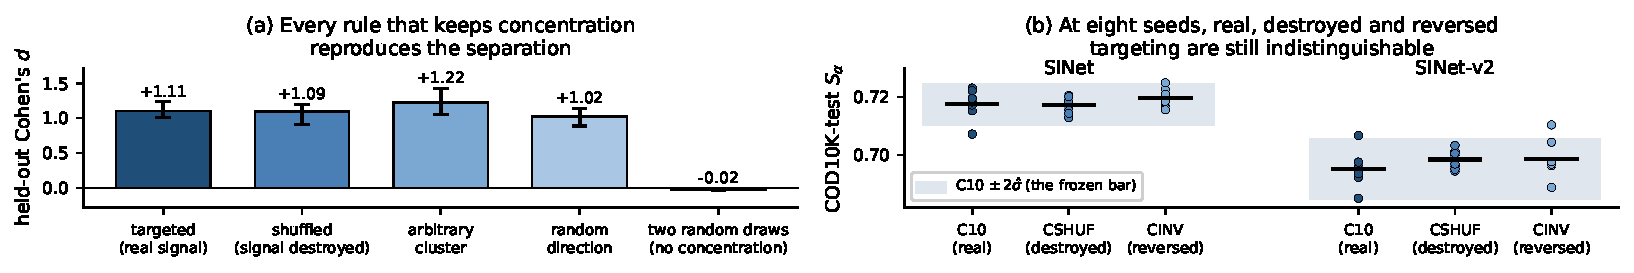
\includegraphics[width=\textwidth]{figs/fig1_thesis.pdf}
\end{center}
\caption{\textbf{(a)} How far a selected set sits from a random set of the same size, in held-out
Cohen's $d$. Every rule that keeps the allocation's \emph{concentration} reproduces the separation; \revB{only a random draw collapses it (a flat quota under the same matching does not; Appendix~\ref{app:shapeoracle}).} Bars are means across the four cells at a budget of $N = 250$; whiskers show the range.
\textbf{(b)} Trained $S_\alpha$ at eight seeds for the three arms that hold concentration fixed and
vary only direction; points are seeds, rules are arm means, the band is the $\pm 2\hat{\sigma}$ bar.
\emph{Sources:} \texttt{c1\_attribution.csv}; \texttt{out/se/abc\_metrics.csv}.}
\label{fig:thesis}
\end{figure}

\revShared{These metrics were not pre-registered and re-decide no verdict. Whether concentration changes accuracy is what our
dose-response experiment was designed to test. It holds the budget at 1,000 images and sets three levels of
concentration: cluster-uniform, the committed shape, and one twice as concentrated. Each concentrated level is
realised with five independent random directions, so direction averages out, and the experiment was pre-registered
with Boundary-IoU on SINet as its primary measure (Table~\ref{tab:cdr}). \cdrverdict{} As delivered, the levels are closer than their quotas (effective numbers of clusters 50, 45 and 41, against 75, 30 and 15; random selection 43), because few foregrounds lie close to most clusters (Section~\ref{sec:discussion}). The planned replication on SINet-v2 was not run, for
lack of compute.}

% =====================================================================
\subsection{Why It Fails}
\label{sec:why}
\revB{Matching and concentration explain} why targeting \emph{looks} the way it does. It does not explain why this loop
could never have delivered the thing it promised, and that has a mechanism, one chain, measured end-to-end before any of the training runs above were scored.

Under every embedding we tried, $k$-means separation peaks at a
silhouette of $0.1600$ and is lower in the other two spaces, far below any conventional threshold
for calling a partition real. So a cluster-wise policy is drawing lines that the data does not
support; \textit{and even where those lines are real, the error does not sit between them.} Only
about a fifth of the endpoint's structural-error variance is between-cluster at all, so four fifths
of what a targeted policy would have to fix is invisible to \emph{any} cluster-level allocation,
however well aimed.

CAMO images are $24.8\%$ of the target pool, and the allocation is not neutral between the two components: $51.5\%$
of the budget lands on them, while the two largest quotas together hold $7$ of the $2026$ images the
paper is scored on (Table~\ref{tab:clustercomp}). ``Allocate by uncertainty'' turns out to be, in substantial part, ``allocate
to CAMO,'' \textit{and the quantity doing the allocating is itself the wrong one.} The
uncertainty score tracks per-pixel error about twice as strongly as it tracks the structural error
the endpoint measures ($+0.8553$ against $+0.4276$), and under whole-image aggregation, that ordering
holds for three families of uncertainty estimators on both architectures, so it is a property of uncertainty-guided allocation
here rather than a quirk of our particular score. Partialling out object area, the most plausible
mechanical explanation, \emph{raises} the structural correlation in every row, the opposite of what the confound predicts. It paints backgrounds and copies objects: the render set is a bijection onto the base foregrounds, and not one
of $8885$ traced objects shows any sign of having been regenerated. The distribution it produces is
narrower than its own input, synthetic images cover $0.13$ to $0.54$ of the real target manifold
($k$-NN recall \revB{at $k = 5$}, Appendix~\ref{app:coverage}\revB{; lower than the input at every $k$ from $3$ to $20$}), while the generator's own source photographs, real
pictures of an entirely different genre, cover $0.71$ to $0.75$. A policy allocating over that pool is choosing among copies.

\textit{One pattern points the other way, and we report it.} Pool \emph{size} may matter where pool
\emph{content} does not: A0, which appends nothing, trails the other arms consistently, reaching a
\textsc{real effect} on the secondary endpoint and two \textsc{inconclusive} verdicts once the
schedule is unpinned. No single step clears its bar, and we claim nothing from it, but it points away
from our conclusion, which is why it is here. Separately, we withdrew one of our own candidate
causes: we suspected the generator's conditioning channel was too narrow to act on a detailed
instruction, read the released source, and found four routes carrying foreground information, with
the dominant one bypassing the bottleneck we had blamed; so the explanation was wrong and is
retired rather than left standing. Appendix~\ref{app:tables} gives the full clustering sweep, the
signal-generality table, and the area control.

% =====================================================================
\subsection{CHAMELEON Is Mostly Training Data}
\label{sec:contamination}
The causes above are about our loop. This one is about the benchmark everyone uses, and it holds
whether or not our loop worked. Fifty of CHAMELEON's $76$ images, $65.8\%$ are the same photographs as images in the
COD10K-train and CAMO training pools, re-encoded, rescaled, or cropped. Forty-four have their
partner in the public COD10K-train split. A model trained on that split has therefore already seen
most of CHAMELEON before being evaluated on it. The standard check does not notice: hashing the
files returns \emph{zero} overlap, and it is not wrong, the copies were re-saved in a different
format, so not one byte matches while every pixel does. Sixteen images resolve neither way \revC{against the training pools} and are
reported \textsc{unchecked} rather than clean, so $50$ is a floor rather than an estimate\revC{. The sixteen are re-encodes
of COD10K-test photographs, as are $32$ of the $76$, so CHAMELEON and COD10K-test are not independent benchmarks
(Appendix~\ref{app:chamext})}.

The count is measured in two tiers (Figure~\ref{fig:cham}). The floor is what a released
same-dimension detector reproduces on any machine: $41$ images whose partner shares their exact
pixel dimensions and differs only by re-encoding. A rescaled or cropped copy leaves its dimension
group and is invisible to that detector, so we recover those by matching keypoints under a geometric
model and then because agreeing on a homography is not the same as being one photograph, warping each candidate into the CHAMELEON frame and measuring the residual. \textit{Nine survive that test}; one cleared the keypoint threshold, failed the residual, and is excluded. Thresholds are calibrated on pairs whose answer is already committed, the finding is verified against a
byte-identical author-sourced release, and the same detector pointed at NC4K flags $0$ of $120$ (Appendix~\ref{app:chamext}).

We expected the contamination to flatter CHAMELEON scores, measured it, and did not find it: all eight difficulty percentiles for the leaked subset fall between $0.448$ and $0.559$. A protocol violation does not need a score advantage to
disqualify a benchmark. Nor do we recommend reporting CHAMELEON on its uncontaminated subset\revC{: of the $26$ images without a training-pool partner,
$24$ are re-encodes of COD10K-test photographs, and we found no duplicate anywhere for only two.} \textit{\revC{A two-image endpoint is not an endpoint}:
report COD10K-test and NC4K instead, and disclose the unchecked share.}\footnote{This is not
hypothetical for the protocol we build on, which designates the real unlabelled COD10K training set
as its target domain. Testing on CHAMELEON, it removes those images from the \emph{source} domain, closing that path but not the target pool, which holds the same $44$. We attribute no intent: the source-side removal shows the authors were alert to leakage, and the target-side path is invisible without a re-encode-tolerant check.} The detector, the pair list, and the clean protocol
are released and run without any of our data.

\begin{figure}[t]
\begin{center}
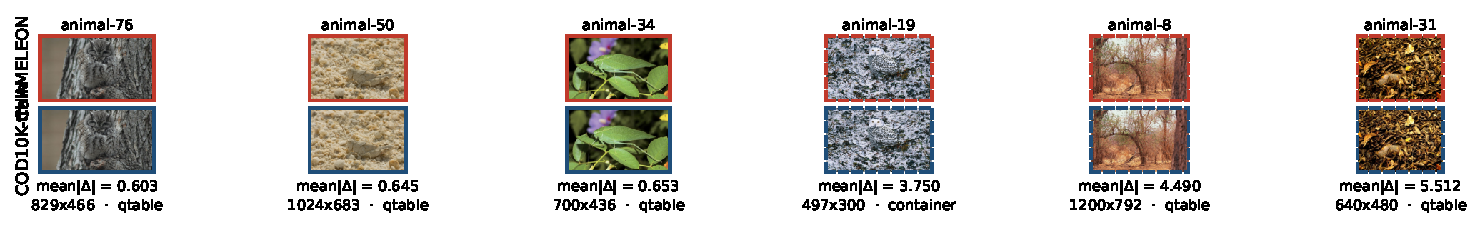
\includegraphics[width=\textwidth]{figs/fig2_pairs.pdf}\\[0.45em]
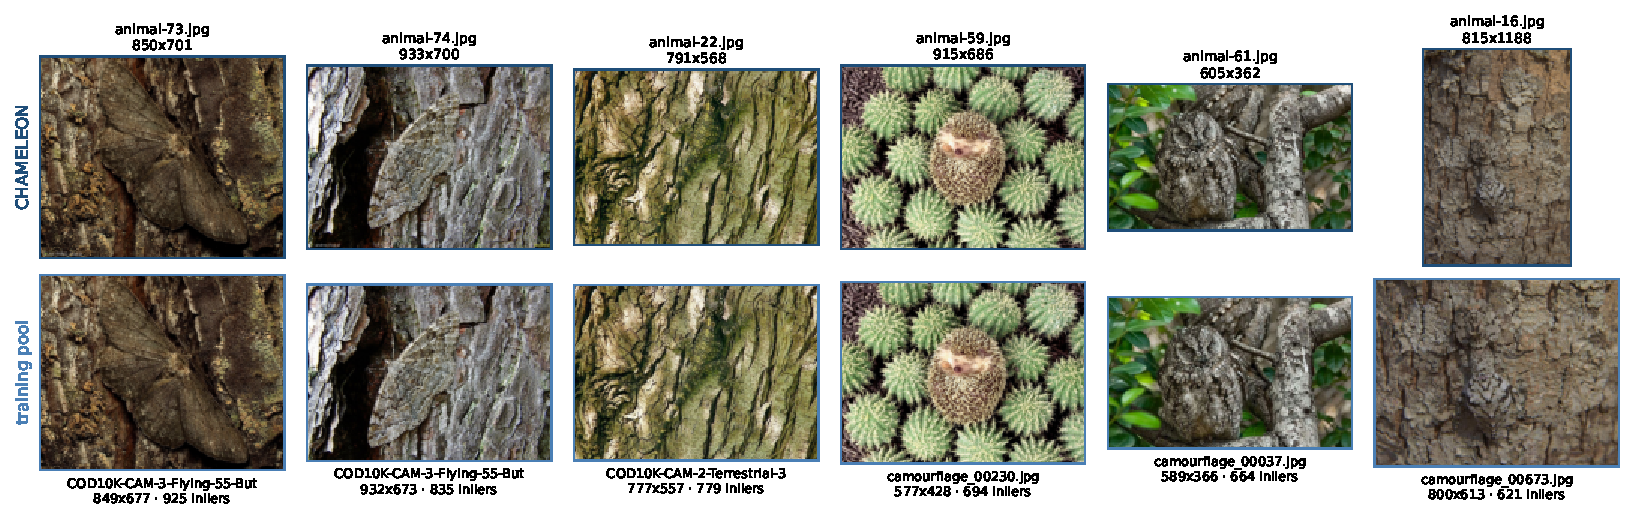
\includegraphics[width=\textwidth]{figs/fig_chameleon_pairs.pdf}
\end{center}
\caption{Two tiers of the same finding. \textit{Top:} six of the $41$ same-dimension
re-encodes the CHAMELEON image above, its training-pool partner below. \textit{Bottom:} six of
the $9$ recovered by geometric adjudication, which the same-dimension detector reports
\textsc{unchecked} because a rescale or a crop moves an image out of its dimension group; note the
differing pixel dimensions in each pair's labels.}
\label{fig:cham}
\end{figure}

% =====================================================================
\section{Discussion}
\label{sec:discussion}
Two kinds of evidence sit underneath this paper and should not be run together. The
\emph{geometric} result is positive, and we state it \revB{plainly: the selector's matching and the budget's concentration}, not the
direction of the uncertainty signal, produce the separation that makes targeted selection look like it works. The \emph{downstream} result is a null under stated sensitivity: \revShared{it excludes an advantage the size of the published method's own gain, a confirmatory campaign bounds the primary gap within $\pm0.005$, and it} does not show that uncertainty guidance cannot work. Four things transfer beyond this setup. \textit{Three checks cost no training and should precede any
cluster-wise allocation:} whether the data separates into clusters at all, what the funded clusters
are made of relative to the pool they are drawn from, and how much of the endpoint's error sits
between clusters rather than within them. \textit{The discriminating control is not a random
baseline} but a same-shape allocation with the signal destroyed inside it, because random selection
differs from targeting in two ways at once. \textit{A null on the endpoint metric does not license a
null on the quantity the acquisition signal was built to move.} And \textit{a real-versus-synthetic AUC near $1.0$ is near-vacuous evidence}: a lossy re-save of the identical images separates at
$0.9928$ (Appendix~\ref{app:coverage}).

The idea still seems reasonable. For it to have a chance, you would need an optimization budget that
grows with the pool rather than one under which added images displace real ones, a foreground supply
not already exhausted \revC{(in this pool a larger budget does not widen the contrast between arms; Appendix~\ref{app:diag})}, a generator wider than its own input, and a target pool that is not a mixture
whose components the signal can tell apart. Nothing here says closed-loop generation cannot work,
only that this build could not have shown that it does. One pattern runs through the method and the
benchmark alike: \textit{a control that returns zero is informative only if it could have returned
something else.}

\revShared{\textit{Scope.} Every conclusion here is bounded to what was tested. The generator is LAKE-RED, run once, offline,
before any training; it never sees the score. Its pool re-uses each of 4,447 HKU-IS foregrounds, already in the base pool, with a new background. Two renders of
the same foreground on different backgrounds share most of their embedding variance (intraclass correlation $0.71$ in
frozen DINOv2 features). In 52 of the 75 target clusters, the nearest available cut-out lies farther from the cluster's
centre than the cluster's median real image, partly a cut-out-versus-photograph difference. The allocation acts on $k = 75$ $k$-means clusters of frozen self-supervised features,
with a budget of $N = 1000$ images, for SINet and SINet-v2 with two-round self-training at a pinned number of
steps, and is read on COD10K-test and NC4K. Whether the null holds at a higher operating point, with some real labels in the pool, was not tested. We tested allocation, not generation: a generator that synthesises new
foregrounds for the hardest clusters, or one steered by the score while it generates, is outside this experiment, and
we make no claim about other generators.} \revB{A modern transformer-based detector is untested as well.}


% =====================================================================
\section{Conclusion}
\label{sec:conclusion}
Under a fixed synthetic-data budget, aiming \revShared{a pool of generated images} at the clusters a model finds hardest \revShared{showed no detectable advantage over} spending it at random. Across $103$ trained runs and five controls that each close a different
route to an artifactual null, the gap stays within noise\revShared{, and a pre-registered confirmatory campaign, incomplete at
16, 15 and 15 of 27 seeds per arm, establishes equivalence within $\pm0.005$ on the primary comparison}. Targeting does change the training set,
but through \revB{matching and} concentration rather than aim\revShared{: same-shape controls show that direction adds nothing
detectable, and a pre-registered dose-response test found no effect of concentration on accuracy. These conclusions hold
for allocation over a fixed LAKE-RED render pool that varies only backgrounds (Section~\ref{sec:discussion})}. Independently,
\revC{at least} $50$ of CHAMELEON's $76$ images are altered copies of COD10K and CAMO training images, which exact
hashing misses. Both findings argue for one practice: before crediting an acquisition rule or
trusting a duplicate check, run the version of the test that could have failed.

\subsection*{AI Use Statement}
We used generative AI tools for the following tasks that require disclosure. \textbf{Implementing
methods:} drafting and refactoring the experiment-driver, training-orchestration, analysis, and
duplicate-detection code. \textbf{Interpreting results:} drafting and editing prose that describes
and frames results, and cross-checking claims in the draft against committed log outputs.
\textbf{Designing or giving feedback on methodology or experiments:} discussion of the control arms
and pre-registration checks reported here, in exchanges directed by the authors, who made every
design decision. We did not use generative AI tools to formulate the hypotheses this work tests, to
select or alter any experimental result, or to clean or reformat datasets. The remaining disclosure
categories (theoretical frameworks, mathematical claims and proofs, translation, and qualitative
data analysis) do not apply. The synthetic training images studied here were produced by the
released LAKE-RED diffusion model (Section~\ref{sec:method}); they are the object of study, not an
assistant use. We additionally used generative AI tools to draft and edit prose, to search and
summarise related literature, and to format references.

The authors reviewed all AI-assisted work, which is itself committed and can be audited rather than
taken on trust. No reported number originates from a language model: every number is emitted by a
committed script and is traceable to a log block, and no result was transcribed by hand. The
decision rules governing every verdict (the arms, the endpoints, the seeds, the noise estimate,
and the verdict bands) were \revB{committed before any result they decide, and all but one before the runs they govern}
(Appendix~\ref{app:method}), with amendments append-only and dated; any analysis outside those rules
is reported as post-hoc and marked as deciding nothing (Tables~\ref{tab:ci_tost}
and~\ref{tab:boundary}). The authors checked every reference against its published version. We take
full responsibility for the content of this work, including text, code, and claims produced with the
aid of generative AI.

\subsection*{Ethics Statement}

This work involves no human subjects and no personally identifying data. It uses four public
research benchmarks for camouflaged object detection: COD10K~\citep{fan2022concealed},
CAMO~\citep{le2019anabranch}, NC4K~\citep{lv2021simultaneously} and
CHAMELEON~\citep{skurowski2018animal} together with the HKU-IS salient-object set as a source
pool and the released LAKE-RED~\citep{zhao2024lakered} generator checkpoint. Each is used for
non-commercial academic research, which is the use its distribution terms provide for, and each is
obtained from its authors' own release rather than redistributed by us; we release no benchmark
imagery, only the derived pair list and detector described below. CHAMELEON, in particular, is an unpublished collection that has become a de facto standard, which is part of why its provenance is worth auditing at all.

Section~\ref{sec:contamination} reports an overlap between two public datasets. We state explicitly
what that measurement does and does not support. It is a measurement of pool membership; it attributes
no intent to any dataset's authors, and we draw the direction of provenance as an inference from
release chronology rather than as a finding. We measured for a score-inflation figure, did not find
one, and do not report one. The one correction we direct at anyone is directed at ourselves: it was
our own protocol that adopted CHAMELEON as an evaluation endpoint without checking whether the
repository we built on ever sanctioned it. We release the detector so that the measurement can be
repeated, contested, or extended by others rather than taken on trust.

\subsection*{Reproducibility Statement}

The decision rules governing every result are \revB{committed before any result they decide, and all but one before the runs they govern}, at the commits
named in Appendix~\ref{app:method}, and amendments to them are append-only and dated. Each experiment
has a committed result document and one or more committed log blocks; each number in this paper is
traceable to such a block or to a committed artifact, and the source line of each table and figure
caption names it. Per-run metrics for all $103$ training runs are in the supplement
(\texttt{rebuild/FinalPaper/results.md})\revShared{; the post-review campaigns add $99$ trained runs (confirmatory $46$,
dose-response $35$, oracle shapes $12$, supervised references $6$), whose records are in the repository's rebuttal
packages} the appendix tabulates the $39$ runs of the two frozen
campaigns and the positive control (Tables~\ref{tab:perrun} and~\ref{tab:perrun-nc4k}), the full
clustering sweep, and the full signal-generality table. The contamination detector is released with an
eight-assertion known-answer self-test that runs without any of our data, alongside the confirmed
pair list, the clean protocol, and the calibration of the geometric extension.

Full code, pretraining scripts, and configurations are available in the anonymized repository: \url{https://anonymous.4open.science/r/AD-35F1/}.

\bibliography{reference}
\bibliographystyle{iclr2027_conference}

\appendix

\ifrevmarked
\paragraph{Revision colours.} In this marked copy, changes made in response to the discussion are coloured by the
reviewer concern they address: \revA{RL5B only, blue}; \revB{Caus only, teal}; \revC{dypE only, purple}; and
\revShared{two or more reviewers, orange}, which overrides the individual colours. Text that is not coloured is
unchanged from the submission or was only moved.
\fi

% =====================================================================
% APPENDIX A -- receives the tab: closest comparison table cut from
% \S2 (artifact G). ViT places no comparison table in related work;
% two sentences in \S2 carry the claim and the table lives here.
% =====================================================================
\section{Additional Related Work}
\label{app:related}

\paragraph{COD benchmarks and detectors.}
The standard camouflaged object detection (COD) evaluation suite comprises COD10K~\citep{fan2022concealed}, a large benchmark
with ten camouflage categories and pixel-accurate masks; CAMO~\citep{le2019anabranch}, which focuses
on man-made camouflage and occlusion; NC4K~\citep{lv2021simultaneously}, received from verified source; and
CHAMELEON~\citep{skurowski2018animal}, an earlier unpublished collection that has become a de facto
standard. The continued use of all four matters for Section~\ref{sec:contamination}: an image shared by a training set and any reported test set contaminates the evaluation for methods using the full suite.
SINet~\citep{fan2020sinet} decomposes COD into search and identification branches, while SINet-v2
\citep{fan2022concealed} adds a neighbour connection decoder for boundary refinement; we use both
off-the-shelf. SegMaR~\citep{jia2022segment} iteratively magnifies and re-processes ambiguous
regions, representing architectural progress outside our allocation experiment. We report the
structure-aware S-measure~\citep{fan2017structure}, enhanced-alignment E-measure
\citep{fan2018enhanced}, and weighted $F_\beta^w$~\citep{margolin2014evaluate} for comparability
with S2R-COD.
\begin{revblock}{RevA}Unsupervised COD avoids masks altogether. RISE~\citep{du2025rise} clusters each training image with frozen DINOv2
features, retrieves prototypes across the whole training set to produce pseudo masks for the 4,040 COD10K and CAMO
training images, and trains SINet-V2 on them with SINet-V2's own recipe, reaching $S_\alpha$ $0.763$ on COD10K-test
and $0.805$ on NC4K. Its detector is the SINet-V2 we use, and its training images are the same 4,040 images our
pipeline uses as unlabelled targets. The gap between the two therefore isolates the source of supervision on those
images, pseudo masks on the real images themselves against synthetic renders plus self-training, far more than any
difference in detector or representation.

% Generated by analysis/make_protocol_table.py from RESULT_TABLES/EXP03_gap_decomposition.json -- do not edit by hand.
\paragraph{Where the absolute gap comes from.} Table~\ref{tab:protocol} places our pipeline beside the method it builds on, RISE, and supervised SINet-V2 under one scorer. Most of the gap to supervised SINet-V2 is the absence of real labels: training our own pipeline on the real masks of the same 4,040 images, in a single round and with our recipe, raises $S_\alpha$ on COD10K-test by $+0.112$ for SINet-V2 and $+0.087$ for SINet over the targeted synthetic-to-real arm, while the official SINet-V2 recipe adds only $+0.008$ on top of that. RISE exceeds our SINet-V2 arm by $+0.068$ on COD10K-test and $+0.056$ on NC4K; since its detector and training images are ours, that gap reflects pseudo masks on the real target images against synthetic renders plus self-training, though without training our recipe on RISE's masks we cannot separate the quality of its supervision from its training recipe. These differences overlap and do not add up to the total gap. None of them changes the comparison this paper is about, which holds the pipeline fixed and varies only the allocation.

\end{revblock}

%% Generated by analysis/make_protocol_table.py from RESULT_TABLES/EXP03_protocol_matched.csv -- do not edit by hand.
\begin{table}[t]
\revfloatcolor{RevA}
\caption{Protocols and accuracy under one scorer and one set of test splits. ``Target images'' is how the 4,040
COD10K and CAMO training images enter training. Our rows are means over seeds; ``re-scored'' rows are released
prediction maps scored with our code, which reproduces every published value within $0.002$; S2R-COD rows are as
published (COD10K only). $E_\phi$ is the mean E-measure. The supervised rows are an upper reference, not a competitor.
R50: ResNet-50; R2-50: Res2Net-50; both ImageNet-pretrained.}
\label{tab:protocol}
\begin{center}
\tiny
\setlength{\tabcolsep}{2.2pt}
\begin{tabular}{@{}llllllcccccc@{}}
\toprule
& & & & & & \multicolumn{3}{c}{COD10K-test} & \multicolumn{3}{c}{NC4K} \\
\cmidrule(lr){7-9}\cmidrule(l){10-12}
Method & Labels & Target images & Detector & Generator & $n$ & $S_\alpha$ & $E_\phi$ & $F_\beta^w$ & $S_\alpha$ & $E_\phi$ & $F_\beta^w$ \\
\midrule
Ours, targeted (C10) & synthetic & unlabelled & SINet (R50) & LAKE-RED & 8 seeds & 0.717 & 0.748 & 0.483 & 0.768 & 0.792 & 0.608 \\
Ours, targeted (C10) & synthetic & unlabelled & SINet-V2 (R2-50) & LAKE-RED & 8 seeds & 0.695 & 0.757 & 0.482 & 0.749 & 0.802 & 0.611 \\
S2R-COD (published) & synthetic & unlabelled & SINet (R50) & HKU-IS synth. & paper & 0.714 & 0.744 & 0.481 & -- & -- & -- \\
S2R-COD (published) & synthetic & unlabelled & SINet-V2 (R2-50) & HKU-IS synth. & paper & 0.684 & 0.757 & 0.476 & -- & -- & -- \\
RISE (released maps) & none & pseudo masks & SINet-V2 (R2-50) & none & re-scored & 0.763 & 0.840 & 0.601 & 0.805 & 0.868 & 0.705 \\
Supervised, our trainer & real masks & labelled & SINet (R50) & none & 3 seeds & 0.805 & 0.829 & 0.607 & 0.840 & 0.864 & 0.717 \\
Supervised, our trainer & real masks & labelled & SINet-V2 (R2-50) & none & 3 seeds & 0.807 & 0.882 & 0.670 & 0.839 & 0.897 & 0.761 \\
SINet-V2 (released maps) & real masks & labelled & SINet-V2 (R2-50) & none & re-scored & 0.815 & 0.887 & 0.680 & 0.847 & 0.903 & 0.770 \\
\bottomrule
\end{tabular}
\end{center}
\end{table}


\paragraph{Synthetic generation and domain adaptation.}
Latent diffusion~\citep{rombach2022high} and DDIM~\citep{song2021denoising} provide the high-resolution
generator and a deterministic sampling schedule inherited by our pipeline. Copy-paste augmentation
\citep{ghiasi2021simple} similarly composes object cutouts with varied backgrounds; LAKE-RED applies
this compositional idea while retrieving background patches. CyCADA~\citep{hoffman2018cycada}, in
contrast, aligns source and target feature distributions with cycle-consistent adversarial training; our loop does not operate at the feature level and instead feeds generator output into a
self-training objective. Other camouflage-image generators exist~\citep{chen2025realcamo}, but they
are outside the experiment, so the reported null is bound to LAKE-RED.

\paragraph{Uncertainty-guided acquisition and self-training.}
FixMatch~\citep{sohn2020fixmatch} couples confidence thresholding with consistency regularisation; our pseudo-labels likewise arise in an inter-round consistency step, but drive a second training
round rather than an online update. Pseudo-labelling~\citep{lee2013pseudo} supplies the hard-target
view of this step. DINOv2~\citep{oquab2024dinov2} and CLIP~\citep{radford2021learning} provide the
frozen representations used for clustering. These choices complement core-set selection
\citep{sener2018active}: the clusters spread the budget, while the disagreement scores determine
which clusters receive more of it. BADGE~\citep{ash2020deep} jointly uses uncertainty and diversity
in gradient-embedding space; our same-shape shuffle in Section~\ref{sec:concentration} is a direct
control for the corresponding entanglement in this allocation.

\paragraph{Benchmark integrity and negative results.}
Dataset-collection procedures can induce shared statistical bias~\citep{torralba2011unbiased}, and
near-duplicate analyses of CIFAR show that visually identical images can cross split
boundaries~\citep{barz2020train}. Related contamination concerns appear in language-model evaluation
\citep{wu2024antileak}; the mechanism differs here, but the need for explicit auditing is shared.
Our pre-registration follows reproducibility guidance~\citep{pineau2021improving} and the case for
publishing disconfirming results~\citep{karl2024position}. Finally, criticisms of learned comparison
measures under resizing and representation choices~\citep{parmar2022aliased,jayasumana2024rethinking}
motivate treating encoding-sensitive probes as diagnostics rather than as clear perceptual evidence.

\paragraph{Where this work sits among budget-steering systems.} Table~\ref{tab:closest} places the
three systems discussed in Section~\ref{sec:related} beside this one. The last column is the point: it records whether a signal-destroying or same-shape control is run, which is what separates an
effect of \emph{aiming} a budget from an effect of \emph{concentrating} it. It is not a claim of
superiority, our own entry records a null.

\begin{table}[t]
\caption{Where this work sits among systems that steer a synthetic-data budget. \emph{Acquisition
signal} is what decides where the budget goes; \emph{generator control} is what the method can
actually vary in the generated image; \emph{diversity control} is what stops the budget piling onto
near-duplicates; \emph{closed-loop} means the downstream model's state feeds back into generation;
\emph{abstention/control} is whether a signal-destroying or same-shape control is run, which is what separates an effect of aiming from an effect of concentrating. The last column is the one this paper argues is missing from the literature, not a claim of superiority; our own entry records a
null.}
\label{tab:closest}
\begin{center}
\small
\setlength{\tabcolsep}{3pt}
\footnotesize
\begin{tabular}{@{}lp{1.75cm}p{1.9cm}p{1.75cm}p{1.35cm}p{1.9cm}@{}}
\toprule
Work & Task & Acquisition signal & Generator control & Closed-loop & Abstention / control \\
\midrule
LAKE-RED~\citep{zhao2024lakered} & COD synthesis & none (uniform) & background only & no & --- \\
S2R-COD~\citep{luo2025s2rcod} & COD adaptation & none (uniform) & background only & pseudo-labels & --- \\
GAUDA~\citep{frisch2025gauda} & surgical seg. & epistemic, per class & image + mask & yes, online & none reported \\
DisCL~\citep{liang2025discl} & long-tail cls. & hardness, per sample & guidance strength & curriculum & none reported \\
SynQuE~\citep{chen2025synque} & dataset ranking & proxy score, per set & n/a (picks sets) & no & none reported \\
\midrule
\textbf{This work} & COD adaptation & disagreement, per cluster & background only & pseudo-labels &
\textbf{same-shape shuffle, rank reversal, oracle} \\
\bottomrule
\end{tabular}
\end{center}
\end{table}

\section{Detailed Method Specification}
\label{app:method}

\paragraph{Training.} SINet~\citep{fan2020sinet} at batch $16$ for $40$ epochs and
SINet-v2~\citep{fan2022concealed} at batch $32$ for $100$ epochs, Adam at $10^{-4}$, images at
$352 \times 352$ with ImageNet normalisation. The exponential-moving-average (EMA) teacher uses momentum $0.996$ under this task
setting. The consistency weights in Equation~\ref{eq:es} are the configured $a = 0.9$, $b = 0.3$
with the unweighted cross-entropy variant, these are the values the trainer sets for this task,
not the loss class's own defaults. ES abbreviates the edge-aware saliency loss of the protocol we
build on; both of its terms are per-pixel means (the $\ell_1$ norm is averaged over pixels), and BCE
takes the teacher's output as its target. The acquisition score uses exactly this unweighted form; the training consistency loss uses the same two terms with a saliency-weighted BCE (per-pixel weight
equal to the teacher's output plus $c = 0.5$). Strong views add random autocontrast and Gaussian blur to the
weak view. \texttt{cudnn.deterministic} is enabled and \texttt{cudnn.benchmark} disabled, which
reduces, and is not claimed to eliminate, kernel nondeterminism.

\paragraph{Seeds and what was held constant.} The committed seeds are $\{42, 43, 45\}$; the seed
expansion of Section~\ref{sec:null} adds $\{46, 47, 48, 49, 50\}$, fixed in writing before its first
run. Across the four-arm campaign's $24$ runs, the base pool is asserted byte-identical against a
hash manifest with $0$ mismatches, both rounds read the unfiltered $4040$-image target set, and every run shares one trainer invocation, checkpoint rule, endpoint set, and deterministic-kernel
setting.

\paragraph{Optimization budget.} Steps per epoch are set by the shorter of the source and target
loaders, which pins them at $253$ (SINet) and $127$ (SINet-v2) in both rounds of every committed run
regardless of pool size, so appended images displace base-pool exposure rather than adding to it.
This is measured per run and asserted rather than assumed. It is not an asymmetry between the arms
that matter: B and C10 hold identical pool sizes and therefore receive identical step counts;
and Section~\ref{sec:null} reports the campaign that removes the pin and re-runs the comparison
without it.

\paragraph{Constructing the falsification arms.} CSHUF's permutation is the \textbf{first} of $64$
pre-declared draws satisfying zero fixed points and $|\rho| \leq 0.10$, chosen by a rule fixed
before the draw and never by inspecting its consequences; its realized rank correlation with the
true score vector is $-0.03351$, against CINV's exact $-1.0$. CINV's single fixed point is
mathematically necessary: at odd $k$ the median-ranked cluster is its own mirror. Because equality
is the \emph{supporting} outcome for these arms, two near-identical arms would manufacture it, so
set distinctness was gated before any GPU time at a Jaccard bound of $0.50$: between $452$ and $511$
of each pair's $1000$ injected images differ, at $2.2$--$2.4\times$ chance overlap.

\paragraph{Allocation rule.} Write $e_j$ for cluster $j$'s score (the mean of Equation~\ref{eq:es}
over its target members), $s_e$ for the population standard deviation of $e_1, \dots, e_k$, and $N$
for the generation budget. Cluster $j$ receives the share
\begin{equation}
p_j \;=\; \frac{\exp\!\big((e_j - \max_i e_i)/(\atemp\, s_e)\big)}{\sum_{l=1}^{k} \exp\!\big((e_l - \max_i e_i)/(\atemp\, s_e)\big)},
\label{eq:alloc}
\end{equation}
and the integer quotas are $\lfloor N p_j \rfloor$ plus one unit to each of the $N - \sum_j \lfloor N p_j \rfloor$
clusters with the largest remainders (ties to the lower index). Dividing by $s_e$ makes $\atemp$
scale-free: on the committed scores $s_e = 0.0101$, and Equation~\ref{eq:alloc} at $\atemp = 1.0$,
$N = 1000$ reproduces all $75$ committed quotas exactly (the ten largest are in
Table~\ref{tab:clustercomp}).

\paragraph{Allocation sweeps.} Stage (iv) matches against a grey-masked cutout rather than a render,
because at selection time, the foreground exists and the render does not. The budget grid is
$N \in \{250, 500, 1000, 2000, 3000, 4447\}$ and the temperature grid over $\atemp$ is extended
until both degenerate ends are reached, concentrated when $\max_j p_j \geq 0.95$, uniform when
total variation from uniform falls below $0.01$ with caps at $\atemp \in [10^{-4}, 10^{3}]$. The
campaign uses $\atemp = 1.0$, $N = 1000$.

\paragraph{Metrics.} $S_\alpha$ at $\alpha = 0.5$ is the primary endpoint metric; mean absolute
error (MAE) on CAMO-250 is the checkpoint-selection metric; $F_\beta^w$ and the E-measure $E_\phi$
\revA{(the mean E-measure over thresholds, the variant SINet-V2 and RISE report)} are computed and reported, but they decide
nothing.
The $F$-measures apply $\beta$ in the non-squared form, so the metric name rather than a formula is what identifies them.

\paragraph{Degrees of freedom.} Each campaign's $\hat{\sigma}$ is pooled within-arm across that
campaign's own arms, at $\mathrm{df} = (\text{arms}) \times (\text{seeds} - 1)$: $8$ for the
three-seed campaigns over four arms, $6$ for the three-arm controls, $4$ for the two-arm positive
control (C10 and MT), and $28$ for the eight-seed expansion. A campaign's bar is never swapped for another campaign's in either direction.

\paragraph{Campaign codes and verdicts.} Table~\ref{tab:trained} labels campaigns ABC (the committed
four-arm campaign: A0, A2, B, C10), SE (seed expansion), OR (oracle, arm CORACLE), FX (unpinned
optimization schedule, arms A0FX, BFX, C10FX), and PC (positive control against a mean-teacher arm,
MT); T2 is the falsification campaign (CSHUF, CINV)\revB{; ORS is the post-review oracle-shape campaign
(Appendix~\ref{app:shapeoracle})}\revShared{; EQ and CDR are the post-review confirmatory-equivalence and dose-response
campaigns (Appendix~\ref{app:diag})}. Every campaign but PC uses the three bands of
Section~\ref{sec:method}. PC's pre-registration names its outcomes \textsc{detected} ($\Delta > 2\hat{\sigma}$
with all seeds agreeing in sign) and \textsc{not detected} ($|\Delta| \le 2\hat{\sigma}$). \revA{The eight-seed expansion
requires at least seven of eight seed-paired differences to agree in sign, a threshold its pre-registration fixed
before its first run: under a fair coin, seven or more of eight has probability $9/256 \approx 0.035$, stricter than
three of three ($0.125$).}

\paragraph{A2 controls one confound.} A2 pairs the authors' original photographs with the
authors' masks, whose mean foreground fraction differs from the raw masks by $0.0058$ on $1000$ of
$5447$ images. This affects $\Delta(\mathrm{B}-\mathrm{A2})$ and is disclosed; it does not touch
$\Delta(\mathrm{C10}-\mathrm{B})$, the decisive gap, since B and C10 share mask provenance, pool
size and render pool.

\paragraph{Pre-registration commits and amendments.} Every decision rule \revB{but one} was committed before the
runs it governs. The four-arm rule is recorded at \texttt{065dac6}, the commit carrying that
campaign's first log block; the falsification campaign's at \texttt{617a2e1}; the signal-generality
check's at \texttt{6efde9f}; the area control's and the positive control's at \texttt{c2114af}\revB{, which was later reset off
the branch and is preserved under the tag \texttt{prereg-ac-pc-c2114af}; the seed expansion's and the
optimization-schedule campaign's at \texttt{a79886a} (2026-09-18 11:48, before either campaign's first run), preserved
under the tag \texttt{prereg-or-fx-se-a79886a}. The oracle campaign's rule was written before any of its scores existed
and committed in the same \texttt{a79886a}, $62$ minutes after its first run had started (first run 10:46, commit
11:48, first score 18:23). The post-review oracle-shape rule (ORS) was committed at \texttt{b21b67c} (2026-11-11), before its
pilot}\revShared{; the confirmatory (EQ) and dose-response (CDR) rules at \texttt{2137849} (2026-11-09), and EQ's one
amendment, which capped $n$ at $27$ per arm and fixed the analysis of an incomplete campaign, at \texttt{808988b}
(2026-11-11), before any EQ run (first CDR run 2026-11-11 18:26; first EQ run 2026-11-13 23:59)}. Three amendments \revShared{to the submitted campaigns} exist, all append-only and dated. Two are reference-tolerance defects of the
same kind: a frozen clause requiring reproduction to better than $10^{-9}$ against a file recording
six decimal places, and in the area control, written by the same author who had just documented
the first, the identical mistake against a file recording four. Both were replaced by exact
agreement at the recorded precision, which is the strictest satisfiable form, and neither altered a
decision threshold. The third marks one verification gate not applicable in scope after it was found
to compare two architectures' signals.


\section{Decisive Gap in Every Cell, and the Bars It Is Read Against}
\label{app:diag}

Table~\ref{tab:trained} reports the primary cell. Table~\ref{tab:allcells} reports all four for
each campaign that attacks the decisive gap. \textbf{Sixteen of sixteen are \textsc{within noise},
and not one reaches half of its bar.}

\begin{table}[h]
\caption{The decisive gap in all four architectures-endpoint cells, per campaign. Each campaign is
read against its \emph{own} pre-registered bar, never another's. \emph{Source:}
\texttt{abc\_verdict.json} and its \texttt{se/}, \texttt{or/}, \texttt{fx/} variants.}
\label{tab:allcells}
\begin{center}
\small
\begin{tabular}{@{}llcccccc@{}}
\toprule
& Cell & $n$ & Gap & $\Delta$ & $2\hat{\sigma}$ & $\times$\,bar & sign \\
\midrule
ABC & SINet $\cdot$ COD10K & 3 & C10$-$B & $+0.0050$ & $0.0179$ & $0.28$ & 3/3 \\
 & SINet $\cdot$ NC4K &  &  & $+0.0021$ & $0.0083$ & $0.25$ & 3/3 \\
 & SINet-v2 $\cdot$ COD10K &  &  & $-0.0004$ & $0.0123$ & $0.03$ & 2/3 \\
 & SINet-v2 $\cdot$ NC4K &  &  & $+0.0009$ & $0.0105$ & $0.09$ & 2/3 \\
\midrule
SE & SINet $\cdot$ COD10K & 8 & C10$-$B & $+0.0024$ & $0.0069$ & $0.34$ & 6/8 \\
 & SINet $\cdot$ NC4K &  &  & $+0.0003$ & $0.0059$ & $0.06$ & 4/8 \\
 & SINet-v2 $\cdot$ COD10K &  &  & $-0.0011$ & $0.0101$ & $0.11$ & 5/8 \\
 & SINet-v2 $\cdot$ NC4K &  &  & $-0.0009$ & $0.0093$ & $0.10$ & 4/8 \\
\midrule
OR & SINet $\cdot$ COD10K & 3 & CORACLE$-$B & $+0.0008$ & $0.0061$ & $0.14$ & 2/3 \\
 & SINet $\cdot$ NC4K &  &  & $-0.0012$ & $0.0047$ & $0.26$ & 2/3 \\
 & SINet-v2 $\cdot$ COD10K &  &  & $+0.0023$ & $0.0093$ & $0.25$ & 2/3 \\
 & SINet-v2 $\cdot$ NC4K &  &  & $+0.0020$ & $0.0080$ & $0.25$ & 2/3 \\
\midrule
FX & SINet $\cdot$ COD10K & 3 & C10FX$-$BFX & $+0.0014$ & $0.0116$ & $0.12$ & 2/3 \\
 & SINet $\cdot$ NC4K &  &  & $+0.0023$ & $0.0107$ & $0.21$ & 2/3 \\
 & SINet-v2 $\cdot$ COD10K &  &  & $-0.0007$ & $0.0100$ & $0.07$ & 1/3 \\
 & SINet-v2 $\cdot$ NC4K &  &  & $-0.0003$ & $0.0122$ & $0.03$ & 1/3 \\
\bottomrule
\end{tabular}
\end{center}
\end{table}

\paragraph{Why the eight-seed bar is wider than the three-seed one.} The seed expansion's arithmetic looks backward. Eight seeds per arm give a truer estimate of the seed-to-seed spread
than three did: the real spread is \emph{larger} than the optimistic three-seed guess, while the gap
itself halved, from $+0.0050$ to $+0.0024$. So the bar sits at $0.0069$ on $28$ degrees of freedom,
not the $0.0034$ the pre-registration projected: $\hat{\sigma}$ is a per-run spread and does not
shrink with seeds, so that projection was an error. The gap now sits inside even the tightest bar
measured on this cell, $0.0055$. The paragraphs below give the per-arm spreads.

%% Values: RL5B STUDENT_RESULTS/RESULT_TABLES/EXP02_SINet_results.md and EXP02_SINet_summary.json.
\begin{table}[h]
\revfloatcolor{RevShared}
\caption{The pre-registered dose-response experiment (SINet, $N = 1000$, $35$ new runs plus the eight-seed B runs).
$\Delta$ is each concentrated level's difference from the dispersed reference (cluster-uniform and random arms,
Boundary-IoU $0.3308$ at threshold $0.5$ on COD10K-test, the primary measure); the bar is $2\hat\sigma = 0.0193$
($\mathrm{df} = 24$). A level counts as an effect only if it clears the bar, at least four of its five random permutations
agree in sign, and the spread between permutations is smaller than the effect. Effective numbers of clusters are
nominal (quota) and delivered (nearest cluster centre of each selected render). The SINet-v2 replication was not run.}
\label{tab:cdr}
\begin{center}
\scriptsize
\setlength{\tabcolsep}{4pt}
\begin{tabular}{@{}lccccccl@{}}
\toprule
Level & Clusters (nom./deliv.) & Runs & $\Delta$ B-IoU & $\times$\,bar & Perms agree & $\Delta S_\alpha$ & Verdict \\
\midrule
Dispersed (uniform, random) & $75$ / $50$ (random $43$) & $5 + 8$ & reference & & & & \\
Committed shape ($\atemp = 1.0$) & $30$ / $45$ & $5 \times 3$ & $-0.0005$ & $0.03$ & $2/5$ & $+0.0004$ & \\
Sharper ($\atemp = 0.758$) & $15$ / $41$ & $5 \times 3$ & $+0.0021$ & $0.11$ & $4/5$ & $+0.0015$ & not supported \\
\bottomrule
\end{tabular}
\end{center}
\end{table}


%% Generated by analysis/make_boundary_table.py from RESULT_TABLES/AN01_boundary_8seed.csv -- do not edit by hand.
\begin{table}[t]
\revfloatcolor{RevShared}
\caption{Boundary-IoU on COD10K-test at eight seeds per arm (binarisation threshold $0.5$; post hoc, decides
nothing). The bar is twice the eight-seed campaign's pooled seed-to-seed spread for this metric; an effect also
needs at least seven of eight seed-paired differences to agree in sign. The last column is the three-seed ratio in
the submitted version. Both SINet contrasts against random that cleared their bars at three seeds are within noise
at eight.}
\label{tab:boundary}
\begin{center}
\scriptsize
\setlength{\tabcolsep}{3.5pt}
\begin{tabular}{@{}llcccccc@{}}
\toprule
Arch. & Contrast & $\Delta$ & bar & $\times$\,bar & sign & verdict (8 seeds) & $\times$\,bar (3 seeds) \\
\midrule
SINet & $\mathrm{C10}-\mathrm{B}$ & $+0.0046$ & $0.0153$ & $0.30$ & 5/8 & \textsc{within noise} & $1.37$ \\
 & $\mathrm{CINV}-\mathrm{B}$ & $+0.0098$ & $0.0153$ & $0.64$ & 7/8 & \textsc{within noise} & $1.34$ \\
 & $\mathrm{CSHUF}-\mathrm{B}$ & $+0.0046$ & $0.0153$ & $0.30$ & 6/8 & \textsc{within noise} & $1.00$ \\
 & $\mathrm{C10}-\mathrm{CSHUF}$ & $+0.0000$ & $0.0153$ & $0.00$ & 4/8 & \textsc{within noise} & $0.37$ \\
 & $\mathrm{C10}-\mathrm{CINV}$ & $-0.0052$ & $0.0153$ & $0.34$ & 4/8 & \textsc{within noise} & $0.04$ \\
\midrule
SINet-v2 & $\mathrm{C10}-\mathrm{B}$ & $+0.0002$ & $0.0095$ & $0.02$ & 4/8 & \textsc{within noise} & $0.16$ \\
 & $\mathrm{CINV}-\mathrm{B}$ & $+0.0033$ & $0.0095$ & $0.34$ & 6/8 & \textsc{within noise} & $0.41$ \\
 & $\mathrm{CSHUF}-\mathrm{B}$ & $+0.0032$ & $0.0095$ & $0.34$ & 5/8 & \textsc{within noise} & $0.20$ \\
 & $\mathrm{C10}-\mathrm{CSHUF}$ & $-0.0031$ & $0.0095$ & $0.33$ & 5/8 & \textsc{within noise} & $0.03$ \\
 & $\mathrm{C10}-\mathrm{CINV}$ & $-0.0031$ & $0.0095$ & $0.33$ & 6/8 & \textsc{within noise} & $0.24$ \\
\bottomrule
\end{tabular}
\end{center}
\end{table}


\paragraph{Why the committed bar is so wide, and why we did not narrow it.} The four-arm campaign
pools its within-arm spread across all four of its arms, and one of them dominates. On the primary
cell the per-arm standard deviations are A0 $0.01727$, A2 $0.00193$, B $0.00181$ and C10 $0.00406$:
\textbf{A0 alone contributes $92.7\%$ of the pooled variance}, and A0 appears in the decisive
comparison not at all. Its instability is unexplained and is reported rather than excluded, because
the bar was pre-registered as a pooled quantity, and re-deriving it after seeing the result is
precisely the move the pre-registration exists to prevent. What we do instead is report the tighter
bars that later campaigns measured on their own arms, and let the reader see all of them.

\paragraph{Three bars, and what each is good for.} Three estimates of the same wobble exist,
and they are not interchangeable. The committed four-arm bar is $0.0179$ and is inflated by A0 as
above. The falsification campaign, pooling over B, C10, CSHUF, and CINV; the arms that actually appear in a decisive gap, yields a measure of $0.0055$ at the same degrees of freedom. The seed expansion
measures $0.0069$ over the same four arms at $28$ degrees of freedom instead of $8$. The asymmetry
that matters is this: where equality is the \emph{supporting} outcome, a tighter bar is
conservative, but here the claim and the null coincide, so a looser bar flatters us. That is why the
paper reads the gap against the tightest defensible bar rather than the widest, and why the seed
expansion's bar, not the committed one, is the sensitivity statement in Section~\ref{sec:null}.

\paragraph{Bar widened when the seeds grew, and the projection it replaced was wrong.} The seed
expansion's pre-registration projected that eight seeds would tighten the bar by
$\sqrt{8/3} \approx 1.63\times$ if the per-arm spreads stayed as measured. That projection was an
error in the pre-registration: $\hat{\sigma}$ is a pooled \emph{per-run} standard deviation, whose
expected value does not depend on the number of seeds, so at unchanged spreads the bar would have
stayed at $0.0055$; a $\sqrt{8/3}$ reduction applies to the standard error of a difference of means,
which the verdict rule does not use. The spreads did not stay put, either. Everyone grew: on the primary cell, B went $0.00181 \rightarrow 0.00251$, C10 $0.00406 \rightarrow 0.00489$, CSHUF
$0.00166 \rightarrow 0.00278$ and CINV $0.00285 \rightarrow 0.00302$. A pooled standard deviation
on eight degrees of freedom is a noisy estimate that lands low as often as high; on twenty-eight, it
is far steadier. So the expansion could never have bought a smaller bar; it bought a trustworthy
one, and showed the three-seed bars to have been optimistic rather than conservative.

%% Generated by analysis/th01_stats.py from rebuild/ABC/out/se/abc_metrics.csv -- do not edit by hand.
\begin{table}[h]
\revfloatcolor{RevShared}
\caption{All sixteen eight-seed contrasts on $S_\alpha$ (moved from the main text; see Table~\ref{tab:equiv}). $\Delta$ is the difference of arm means
(eight seeds each); intervals are Welch. A contrast is \emph{detected} if its 95\% interval excludes
zero, and \emph{equivalent} if its 90\% interval lies inside $\pm0.005$ (TOST~\citep{lakens2017equivalence}, bold
$p<0.05$); \emph{neither} is a failure to detect an effect at this precision, not evidence of equivalence. The
smallest margin at which a contrast would be equivalent is the larger absolute end of its 90\% interval. The margin was chosen after the experiments, and no entry changes a pre-registered verdict.}
\label{tab:ci_tost}
\begin{center}
\scriptsize
\setlength{\tabcolsep}{3pt}
\begin{tabular}{@{}llccccl@{}}
\toprule
Cell & Contrast & $\Delta$ & 95\% CI & 90\% CI & TOST $p$ & Label \\
\midrule
SINet, COD10K & $\mathrm{C10}-\mathrm{B}$ & $+0.0024$ & $[-0.0020, +0.0067]$ & $[-0.0012, +0.0059]$ & 0.101 & neither \\
 & $\mathrm{C10}-\mathrm{CSHUF}$ & $+0.0003$ & $[-0.0041, +0.0047]$ & $[-0.0033, +0.0039]$ & \textbf{0.019} & equivalent \\
 & $\mathrm{C10}-\mathrm{CINV}$ & $-0.0021$ & $[-0.0066, +0.0023]$ & $[-0.0057, +0.0015]$ & 0.091 & neither \\
 & $\mathrm{CSHUF}-\mathrm{CINV}$ & $-0.0024$ & $[-0.0055, +0.0007]$ & $[-0.0050, +0.0001]$ & \textbf{0.049} & equivalent \\
\midrule
SINet, NC4K & $\mathrm{C10}-\mathrm{B}$ & $+0.0003$ & $[-0.0033, +0.0040]$ & $[-0.0027, +0.0033]$ & \textbf{0.008} & equivalent \\
 & $\mathrm{C10}-\mathrm{CSHUF}$ & $+0.0007$ & $[-0.0029, +0.0042]$ & $[-0.0022, +0.0036]$ & \textbf{0.011} & equivalent \\
 & $\mathrm{C10}-\mathrm{CINV}$ & $-0.0031$ & $[-0.0067, +0.0006]$ & $[-0.0060, -0.0001]$ & 0.131 & neither \\
 & $\mathrm{CSHUF}-\mathrm{CINV}$ & $-0.0037$ & $[-0.0064, -0.0011]$ & $[-0.0059, -0.0016]$ & 0.162 & detected \\
\midrule
SINet-v2, COD10K & $\mathrm{C10}-\mathrm{B}$ & $-0.0011$ & $[-0.0067, +0.0045]$ & $[-0.0057, +0.0035]$ & 0.076 & neither \\
 & $\mathrm{C10}-\mathrm{CSHUF}$ & $-0.0033$ & $[-0.0087, +0.0020]$ & $[-0.0077, +0.0010]$ & 0.252 & neither \\
 & $\mathrm{C10}-\mathrm{CINV}$ & $-0.0035$ & $[-0.0101, +0.0031]$ & $[-0.0089, +0.0020]$ & 0.314 & neither \\
 & $\mathrm{CSHUF}-\mathrm{CINV}$ & $-0.0001$ & $[-0.0057, +0.0054]$ & $[-0.0047, +0.0044]$ & \textbf{0.040} & equivalent \\
\midrule
SINet-v2, NC4K & $\mathrm{C10}-\mathrm{B}$ & $-0.0009$ & $[-0.0068, +0.0049]$ & $[-0.0057, +0.0038]$ & 0.079 & neither \\
 & $\mathrm{C10}-\mathrm{CSHUF}$ & $-0.0023$ & $[-0.0078, +0.0031]$ & $[-0.0068, +0.0021]$ & 0.153 & neither \\
 & $\mathrm{C10}-\mathrm{CINV}$ & $-0.0043$ & $[-0.0102, +0.0016]$ & $[-0.0091, +0.0006]$ & 0.394 & neither \\
 & $\mathrm{CSHUF}-\mathrm{CINV}$ & $-0.0019$ & $[-0.0061, +0.0022]$ & $[-0.0053, +0.0015]$ & 0.066 & neither \\
\bottomrule
\end{tabular}
\end{center}
\end{table}


\begin{revblock}{RevShared}
\paragraph{The confirmatory equivalence campaign (EQ).} It was pre-registered after review, with Welch TOST at
$\pm 0.005$ $S_\alpha$ on SINet $\cdot$ COD10K-test as its primary test (H1, C10$-$B) and C10$-$CSHUF as its secondary
test (H1b). A power analysis gave $29$ seeds per arm for power $0.80$ at a true $\Delta = +0.0024$; the first amendment
capped this at $27$ (seeds $101$--$127$, power $0.78$) before any run and fixed the rule for a campaign the cutoff
interrupts: every completed run of each arm is analysed, none is dropped, and the result is labelled incomplete.
Repeated power outages left $46$ of the $81$ runs complete, $16$ (B, seeds $101$--$116$), $15$ (C10) and $15$ (CSHUF,
both seeds $101$--$115$). Run-to-run spread is larger than in the eight-seed campaign ($\hat\sigma = 0.0064$ against
$0.0034$), and it tracks how many target images each run's self-training round pseudo-labels ($r = 0.74$ across runs).
Two checks run after the cutoff are exploratory and decide nothing: same-seed re-training shows that training is not
reproducible run to run (one re-train moved from $0.6933$ to $0.7214$), and leaving out either of the two runs with the
fewest pseudo-labels changes neither verdict.
\end{revblock}

%% Values: dypE STUDENT_RESULTS/RESULT_TABLES/TH-01_paired_inference.csv. Checked by tools/verify_numbers.py.
\begin{table}[h]
\revfloatcolor{RevC}
\caption{Targeted minus random ($S_\alpha$) at eight seeds, paired by training seed beside the Welch analysis (post hoc;
decides nothing). Pairing does not sharpen the comparison, because B redraws its images at every seed: on the primary
cell the paired scores are uncorrelated ($r = -0.04$), the targeted arm is ahead on $6$ of $8$ seeds (exact sign-flip
$p = 0.29$), and the smallest margin at which the paired test would show equivalence is $\pm 0.0061$.}
\label{tab:paired}
\begin{center}
\scriptsize
\setlength{\tabcolsep}{4pt}
\begin{tabular}{@{}lccc@{}}
\toprule
Cell & Welch 95\% CI & Paired 95\% CI & Paired TOST $p$ ($\pm0.005$) \\
\midrule
SINet, COD10K (primary) & $[-0.0020, +0.0067]$ & $[-0.0023, +0.0070]$ & $0.111$ \\
SINet, NC4K & $[-0.0033, +0.0040]$ & $[-0.0038, +0.0045]$ & $\mathbf{0.016}$ \\
SINet-v2, COD10K & $[-0.0067, +0.0045]$ & $[-0.0081, +0.0059]$ & $0.114$ \\
SINet-v2, NC4K & $[-0.0068, +0.0049]$ & $[-0.0077, +0.0058]$ & $0.100$ \\
\bottomrule
\end{tabular}
\end{center}
\end{table}


\paragraph{The interval at three seeds, and why it was left out of the main text.} A Welch interval on the two
arms actually compared, at the committed three seeds, places the decisive gap in
$[-0.0035, +0.0136]$ and excludes the reference effect. The eight-seed interval supersedes it
reported in Section~\ref{sec:null} and is recorded here only for continuity with the committed
account: at roughly $2.8$ degrees of freedom, its exclusion held by a margin too thin to lean on,
which is exactly the weakness the seed expansion removes.

\begin{revblock}{RevShared}
% Generated by analysis/make_boundary_sweep.py from RESULT_TABLES/AN01_boundary_8seed.csv -- do not edit by hand.
\paragraph{Boundary metrics: the binarisation sweep in full.} Boundary metrics binarise a prediction where $S_\alpha$ does not, so a threshold could create or hide an effect. At the committed three seeds, swept over thresholds $0.4 / 0.5 / 0.6$ on SINet Boundary-IoU~\citep{cheng2021boundary}, $\Delta(\mathrm{C10}-\mathrm{B})$ sat at $1.39 / 1.37 / 1.23\times$ its bar and $\Delta(\mathrm{CINV}-\mathrm{B})$ at $1.25 / 1.34 / 1.26\times$, while the two direction contrasts never exceeded $0.52\times$ and $0.14\times$. At eight seeds the same sweep gives $0.34 / 0.30 / 0.26\times$ and $0.67 / 0.64 / 0.59\times$, and the direction contrasts stay at or below $0.34\times$: every contrast is within noise at every threshold (Table~\ref{tab:boundary} shows threshold $0.5$). The threshold changes neither reading; the seed count does.

\end{revblock}

\begin{revblock}{RevC}
\paragraph{Architecture, multiplicity and domain mix.} Tested directly, the difference between the architectures'
Boundary-IoU gains over random (threshold $0.5$, COD10K-test) is $+0.0044$ (95\% CI $[-0.0075, +0.0163]$, $p = 0.43$)
for the targeted arm and $+0.0065$ ($[-0.0001, +0.0131]$, $p = 0.053$) for the reversed arm, so the interaction is not
resolved either way: we cannot say the two architectures differ, or that they agree. None of the $140$ eight-seed
contrasts (two boundary metrics at three thresholds and $S_\alpha$, on both architectures and endpoints) survives a Holm
correction; the smallest adjusted $p$ is $0.50$. On $S_\alpha$ the reversed arm also leads random on SINet $\cdot$
COD10K-test ($+0.0045$, paired 95\% CI $[+0.0015, +0.0074]$), inside its bar ($0.65\times$) and not after correction.
One candidate explanation, untested: the three same-shape arms put $53\%$, $29\%$ and $20\%$ of their budget on CAMO
images (targeted, shuffled, reversed), and neither endpoint contains CAMO images.
\end{revblock}

\paragraph{How much the trained comparison is attenuated.} The trained half of the concentration
result is diluted three times over, and we disclose it because the attenuation biases toward the
null we report. Injected images are $1000$ of $5447$ pairs, or $18.4\%$ of the pool; under the
committed schedule, the pinned step count dilutes their exposure further; and \revC{how many injected images differ depends
on the comparison. The three concentrated arms share about half of theirs ($45$--$51\%$ differ, $8.3$--$9.4\%$ of the
training pool). Targeted and random selection share far less, $209$--$246$ of $1000$ per seed, close to the $225$
expected by chance, so $77\%$ of injected images and $14.1\%$ of the training pool differ in the decisive comparison.
Under the pinned schedule an epoch draws $4048$ of the $5447$ source images, so images present only in the targeted arm
are about $14\%$ of source draws in round one and $10\%$ in round two (expected values; the sampler order was not
logged). Between rounds each arm also appends its own pseudo-labelled target images, and the targeted and random sets
of these overlap only at Jaccard $0.58$--$0.68$, a second difference that follows from the first round and is reported
rather than adjusted away. A larger budget does not widen the decisive contrast in this pool: the differing share is
$17.2\%$ at $2000$ images ($1.22\times$ the committed one), $13.1\%$ at $3000$ and $0$ at $4447$, because random
selection draws from the same finite foreground set that targeting ranks; a preflight fixed in advance required
$1.5\times$ before any training, and it failed, so nothing was trained.} Two of the
three \revC{attenuations} are now measured rather than argued: the optimization-schedule campaign removes the pin and
the decisive gap \emph{shrinks}, and the seed expansion raises the degrees of freedom behind the
bar from $8$ to $28$. What remains is the third, which is a property of comparing two arms that
share their whole base pool \revC{and, for the concentrated arms, about half of their injected images}.

\section{Supplementary Tables}
\label{app:tables}

\begin{table}[h]
\caption{Full clustering sweep over the target set: silhouette (mean over 10 $k$-means seeds),
bootstrap ARI and seed ARI, for every $k$ in the declared grid and all three embedding spaces.
The principled $k$ per space is \textbf{bold}. No $k$ in any space reaches a silhouette conventionally
regarded as well-separated structure, and \texttt{clipL224} falls almost monotonically, so its selection
criterion returns the grid edge rather than an interior maximum --- recorded as a FAIL of the declared
guard. \emph{Source:} \texttt{b1\_k\_sweep\_*.csv};
block \texttt{EXP B1} \#3 @ \texttt{results/REBUILD\_LOG.txt:922}.}
\label{tab:silhouette}
\begin{center}\small
\begin{tabular}{rcccccccccc}
\toprule
& \multicolumn{3}{c}{\texttt{dinoL224}} & \multicolumn{3}{c}{\texttt{dinoL518}} & \multicolumn{3}{c}{\texttt{clipL224}} \\
\cmidrule(lr){2-4}\cmidrule(lr){5-7}\cmidrule(lr){8-10}
$k$ & sil. & bs.ARI & sd.ARI & sil. & bs.ARI & sd.ARI & sil. & bs.ARI & sd.ARI \\
\midrule
5 & 0.0538 & 0.712 & 0.795 & 0.0566 & 0.624 & 0.732 & \textbf{0.0568} & 0.953 & 0.983 \\
10 & 0.0868 & 0.676 & 0.709 & 0.0923 & 0.598 & 0.770 & 0.0550 & 0.692 & 0.805 \\
15 & 0.1053 & 0.608 & 0.714 & 0.1152 & 0.573 & 0.592 & 0.0486 & 0.575 & 0.670 \\
20 & 0.1180 & 0.629 & 0.693 & 0.1326 & 0.506 & 0.524 & 0.0486 & 0.635 & 0.646 \\
30 & 0.1378 & 0.596 & 0.642 & 0.1527 & 0.539 & 0.617 & 0.0488 & 0.609 & 0.631 \\
50 & \textbf{0.1465} & 0.610 & 0.615 & 0.1556 & 0.579 & 0.600 & 0.0448 & 0.498 & 0.549 \\
75 & 0.1457 & 0.588 & 0.627 & \textbf{0.1600} & 0.579 & 0.616 & 0.0396 & 0.463 & 0.477 \\
100 & 0.1419 & 0.608 & 0.637 & 0.1557 & 0.583 & 0.601 & 0.0382 & 0.419 & 0.452 \\
150 & 0.1367 & 0.630 & 0.636 & 0.1507 & 0.618 & 0.625 & 0.0357 & 0.380 & 0.409 \\
\bottomrule
\end{tabular}
\end{center}
\end{table}

\begin{table}[h]
\caption{Full signal-generality measurement, all 16 rows: four signal variants across three signal
families, two architectures, two aggregations. $\rho$ at the committed seed, $\pm$ sd over 10
$k$-means seeds. The whole-image block passes the pre-registered ordering $8/8$; the boundary block
passes $2/8$ with four rows going negative, an outcome outside the pre-registered interpretation
space, reported as it fell. \emph{Source:} \texttt{rebuild/T2C/out/t2c\_table.csv}; block
\texttt{EXP T2C} @ \texttt{results/REBUILD\_LOG.txt:2550}.}
\label{tab:t2cfull}
\begin{center}\footnotesize
\setlength{\tabcolsep}{1.5pt}
\begin{tabular}{llcccccc}
\toprule
arch & signal & agg. & $\rho(\mathrm{MAE})$ & $\rho(1-S_\alpha)$ & $\rho(1-\mathrm{IoU})$ & order & seeds \\
\midrule
SINet-v2 & ES & whole & $+0.7070 \pm 0.0404$ & $+0.5628 \pm 0.0359$ & $+0.4591 \pm 0.0315$ & PASS & 10/10 \\
SINet-v2 & ensemble A0 & whole & $+0.6191 \pm 0.0675$ & $+0.5483 \pm 0.0409$ & $+0.4540 \pm 0.0451$ & PASS & 9/10 \\
SINet-v2 & ensemble CSHUF & whole & $+0.5576 \pm 0.0690$ & $+0.4488 \pm 0.0580$ & $+0.3370 \pm 0.0577$ & PASS & 10/10 \\
SINet-v2 & entropy & whole & $+0.7393 \pm 0.0309$ & $+0.5404 \pm 0.0408$ & $+0.4070 \pm 0.0395$ & PASS & 10/10 \\
SINet-v2 & ES & bound & $-0.5485 \pm 0.0745$ & $-0.1146 \pm 0.0675$ & $+0.0537 \pm 0.0558$ & FAIL & 0/10 \\
SINet-v2 & ensemble A0 & bound & $-0.1960 \pm 0.0524$ & $+0.0425 \pm 0.0410$ & $+0.0933 \pm 0.0396$ & FAIL & 0/10 \\
SINet-v2 & ensemble CSHUF & bound & $-0.2527 \pm 0.0668$ & $-0.0591 \pm 0.0609$ & $-0.0011 \pm 0.0579$ & FAIL & 0/10 \\
SINet-v2 & entropy & bound & $+0.4208 \pm 0.0356$ & $+0.4182 \pm 0.0455$ & $+0.3605 \pm 0.0470$ & PASS & 8/10 \\
SINet & ES & whole & $+0.6284 \pm 0.0381$ & $+0.3433 \pm 0.0301$ & $+0.2613 \pm 0.0383$ & PASS & 10/10 \\
SINet & ensemble A0 & whole & $+0.6028 \pm 0.0466$ & $+0.2698 \pm 0.0487$ & $+0.1491 \pm 0.0560$ & PASS & 10/10 \\
SINet & ensemble CSHUF & whole & $+0.5212 \pm 0.0564$ & $+0.4006 \pm 0.0459$ & $+0.3361 \pm 0.0447$ & PASS & 10/10 \\
SINet & entropy & whole & $+0.5892 \pm 0.0368$ & $+0.4267 \pm 0.0277$ & $+0.3588 \pm 0.0351$ & PASS & 10/10 \\
SINet & ES & bound & $-0.0012 \pm 0.0481$ & $-0.0567 \pm 0.0500$ & $-0.0554 \pm 0.0479$ & FAIL & 8/10 \\
SINet & ensemble A0 & bound & $+0.3633 \pm 0.0605$ & $+0.2910 \pm 0.0509$ & $+0.2215 \pm 0.0513$ & PASS & 10/10 \\
SINet & ensemble CSHUF & bound & $+0.3175 \pm 0.0637$ & $+0.3857 \pm 0.0381$ & $+0.3770 \pm 0.0322$ & FAIL & 2/10 \\
SINet & entropy & bound & $+0.2434 \pm 0.0414$ & $+0.2492 \pm 0.0540$ & $+0.2432 \pm 0.0563$ & FAIL & 6/10 \\
\bottomrule
\end{tabular}
\end{center}
\end{table}

\begin{table}[h]
\caption{The area control (\texttt{EXP AC}). First-order partial Spearman on the same cluster
partition and floors as the committed measurement. $z_{\mathrm{obj}}$ = per-cluster mean object area
on the endpoint side; $z_{\mathrm{unc}}$ = per-cluster mean uncertain-region area on the target side.
Ordering survives $7/8$ and $6/8$ against a floor of $6/8$ declared before the run. Note that
partialling object area \emph{raises} $\rho(1-S_\alpha)$ in every row --- the opposite of the
confound's prediction. \emph{Source:} \texttt{rebuild/AC/out/ac\_table.csv}; block \texttt{EXP AC} @
\texttt{results/REBUILD\_LOG.txt:2612}.}
\label{tab:areacontrol}
\begin{center}\small
\begin{tabular}{llcccccc}
\toprule
 & & \multicolumn{2}{c}{raw} & \multicolumn{2}{c}{$|\,z_{\mathrm{obj}}$} & \multicolumn{2}{c}{$|\,z_{\mathrm{unc}}$} \\
\cmidrule(lr){3-4}\cmidrule(lr){5-6}\cmidrule(lr){7-8}
arch & signal & MAE & $1-S_\alpha$ & MAE & $1-S_\alpha$ & MAE & $1-S_\alpha$ \\
\midrule
SINet & ES & $+0.6284$ & $+0.3433$ & $+0.5761$ & $+0.4988$ & $+0.5518$ & $+0.3897$ \\
SINet & entropy & $+0.5892$ & $+0.4267$ & $+0.5505$ & $+0.5517$ & $+0.5060$ & $+0.4426$ \\
SINet & ensemble A0 & $+0.6028$ & $+0.2698$ & $+0.5411$ & $+0.4301$ & $+0.5603$ & $+0.2583$ \\
SINet & ensemble CSHUF & $+0.5212$ & $+0.4006$ & $+0.5002$ & $+0.4857$ & $+0.4857$ & $+0.3937$ \\
SINet-v2 & ES & $+0.7070$ & $+0.5628$ & $+0.7062$ & $+0.6272$ & $+0.4457$ & $+0.4744$ \\
SINet-v2 & entropy & $+0.7393$ & $+0.5404$ & $+0.7134$ & $+0.6546$ & $+0.5369$ & $+0.4266$ \\
SINet-v2 & ensemble A0 & $+0.6191$ & $+0.5483$ & $+0.6245$ & $+0.5969$ & $+0.4355$ & $+0.4488$ \\
SINet-v2 & ensemble CSHUF & $+0.5576$ & $+0.4488$ & $+0.5344$ & $+0.5209$ & $+0.4482$ & $+0.3615$ \\
\midrule
\multicolumn{2}{l}{ordering holds} & \multicolumn{2}{c}{$8/8$} & \multicolumn{2}{c}{$7/8$} & \multicolumn{2}{c}{$6/8$} \\
\bottomrule
\end{tabular}
\end{center}
\end{table}

\begin{table}[p]
\caption{Per-run metrics at full recorded precision, COD10K-test endpoint, for every run of the two
frozen campaigns and the mean-teacher positive control --- $39$ of the $103$ training runs in this
work; Table~\ref{tab:perrun-nc4k} gives the same runs on NC4K. Arms B and C10 appear once; they were
re-scored, not re-trained, for the falsification campaign and reproduced their committed values
exactly at six decimal places. \emph{Source:} \texttt{rebuild/ABC/out/abc\_metrics.csv},
\texttt{out/t2/abc\_metrics.csv} and \texttt{rebuild/PC/out/pc\_metrics.csv}; blocks
\texttt{EXP ABC} \#3 and \texttt{EXP T2} \#3.}
\label{tab:perrun}
\begin{center}\small
\begin{tabular}{llllcc}
\toprule
arch & arm & seed & endpoint & $S_\alpha$ & MAE \\
\midrule
SINet & A0 & 42 & COD10K & 0.715086 & 0.074960 \\
SINet & A0 & 43 & COD10K & 0.681706 & 0.077044 \\
SINet & A0 & 45 & COD10K & 0.706058 & 0.077347 \\
SINet & A2 & 42 & COD10K & 0.705507 & 0.075994 \\
SINet & A2 & 43 & COD10K & 0.708334 & 0.078489 \\
SINet & A2 & 45 & COD10K & 0.709196 & 0.080858 \\
SINet & B & 42 & COD10K & 0.711554 & 0.076085 \\
SINet & B & 43 & COD10K & 0.713632 & 0.076278 \\
SINet & B & 45 & COD10K & 0.715155 & 0.075917 \\
SINet & C10 & 42 & COD10K & 0.717165 & 0.073184 \\
SINet & C10 & 43 & COD10K & 0.723034 & 0.075136 \\
SINet & C10 & 45 & COD10K & 0.715243 & 0.078355 \\
SINet & CINV & 42 & COD10K & 0.722612 & 0.073910 \\
SINet & CINV & 43 & COD10K & 0.717343 & 0.077323 \\
SINet & CINV & 45 & COD10K & 0.718084 & 0.073607 \\
SINet & CSHUF & 42 & COD10K & 0.718602 & 0.074840 \\
SINet & CSHUF & 43 & COD10K & 0.716974 & 0.077678 \\
SINet & CSHUF & 45 & COD10K & 0.715291 & 0.079340 \\
SINet & MT & 42 & COD10K & 0.699633 & 0.093377 \\
SINet & MT & 43 & COD10K & 0.699167 & 0.087571 \\
SINet & MT & 45 & COD10K & 0.697503 & 0.091322 \\
SINetv2 & A0 & 42 & COD10K & 0.688813 & 0.091691 \\
SINetv2 & A0 & 43 & COD10K & 0.678740 & 0.095147 \\
SINetv2 & A0 & 45 & COD10K & 0.699883 & 0.085756 \\
SINetv2 & A2 & 42 & COD10K & 0.691914 & 0.089186 \\
SINetv2 & A2 & 43 & COD10K & 0.688977 & 0.094524 \\
SINetv2 & A2 & 45 & COD10K & 0.695414 & 0.087455 \\
SINetv2 & B & 42 & COD10K & 0.698340 & 0.092242 \\
SINetv2 & B & 43 & COD10K & 0.689481 & 0.089883 \\
SINetv2 & B & 45 & COD10K & 0.697385 & 0.087132 \\
SINetv2 & C10 & 42 & COD10K & 0.692321 & 0.093395 \\
SINetv2 & C10 & 43 & COD10K & 0.696328 & 0.090749 \\
SINetv2 & C10 & 45 & COD10K & 0.695360 & 0.089182 \\
SINetv2 & CINV & 42 & COD10K & 0.697008 & 0.088438 \\
SINetv2 & CINV & 43 & COD10K & 0.696331 & 0.087293 \\
SINetv2 & CINV & 45 & COD10K & 0.697605 & 0.090189 \\
SINetv2 & CSHUF & 42 & COD10K & 0.701269 & 0.087506 \\
SINetv2 & CSHUF & 43 & COD10K & 0.694490 & 0.087305 \\
SINetv2 & CSHUF & 45 & COD10K & 0.696218 & 0.089485 \\
\bottomrule
\end{tabular}
\end{center}
\end{table}

\begin{table}[p]
\caption{Per-run metrics at full recorded precision, NC4K endpoint, for the same $39$ runs as
Table~\ref{tab:perrun}. \emph{Source:} as Table~\ref{tab:perrun}.}
\label{tab:perrun-nc4k}
\begin{center}\small
\begin{tabular}{llllcc}
\toprule
arch & arm & seed & endpoint & $S_\alpha$ & MAE \\
\midrule
SINet & A0 & 42 & NC4K & 0.765121 & 0.085752 \\
SINet & A0 & 43 & NC4K & 0.751545 & 0.088874 \\
SINet & A0 & 45 & NC4K & 0.757700 & 0.090228 \\
SINet & A2 & 42 & NC4K & 0.760908 & 0.088385 \\
SINet & A2 & 43 & NC4K & 0.762933 & 0.087466 \\
SINet & A2 & 45 & NC4K & 0.765789 & 0.090892 \\
SINet & B & 42 & NC4K & 0.764108 & 0.087897 \\
SINet & B & 43 & NC4K & 0.768972 & 0.085001 \\
SINet & B & 45 & NC4K & 0.767632 & 0.088175 \\
SINet & C10 & 42 & NC4K & 0.765296 & 0.086273 \\
SINet & C10 & 43 & NC4K & 0.771241 & 0.085305 \\
SINet & C10 & 45 & NC4K & 0.770503 & 0.086622 \\
SINet & CINV & 42 & NC4K & 0.774697 & 0.083144 \\
SINet & CINV & 43 & NC4K & 0.774114 & 0.084030 \\
SINet & CINV & 45 & NC4K & 0.768136 & 0.084570 \\
SINet & CSHUF & 42 & NC4K & 0.766713 & 0.085734 \\
SINet & CSHUF & 43 & NC4K & 0.767983 & 0.085825 \\
SINet & CSHUF & 45 & NC4K & 0.767229 & 0.089734 \\
SINet & MT & 42 & NC4K & 0.752869 & 0.108067 \\
SINet & MT & 43 & NC4K & 0.746708 & 0.101192 \\
SINet & MT & 45 & NC4K & 0.749400 & 0.104323 \\
SINetv2 & A0 & 42 & NC4K & 0.745691 & 0.092348 \\
SINetv2 & A0 & 43 & NC4K & 0.736067 & 0.099838 \\
SINetv2 & A0 & 45 & NC4K & 0.751473 & 0.092634 \\
SINetv2 & A2 & 42 & NC4K & 0.747102 & 0.093372 \\
SINetv2 & A2 & 43 & NC4K & 0.743257 & 0.097429 \\
SINetv2 & A2 & 45 & NC4K & 0.753292 & 0.090255 \\
SINetv2 & B & 42 & NC4K & 0.753317 & 0.097475 \\
SINetv2 & B & 43 & NC4K & 0.743653 & 0.095901 \\
SINetv2 & B & 45 & NC4K & 0.748868 & 0.091476 \\
SINetv2 & C10 & 42 & NC4K & 0.748534 & 0.096669 \\
SINetv2 & C10 & 43 & NC4K & 0.750839 & 0.097324 \\
SINetv2 & C10 & 45 & NC4K & 0.749305 & 0.092402 \\
SINetv2 & CINV & 42 & NC4K & 0.752956 & 0.095453 \\
SINetv2 & CINV & 43 & NC4K & 0.753600 & 0.089466 \\
SINetv2 & CINV & 45 & NC4K & 0.753833 & 0.094549 \\
SINetv2 & CSHUF & 42 & NC4K & 0.754154 & 0.093821 \\
SINetv2 & CSHUF & 43 & NC4K & 0.750543 & 0.094270 \\
SINetv2 & CSHUF & 45 & NC4K & 0.749500 & 0.095273 \\
\bottomrule
\end{tabular}
\end{center}
\end{table}


\begin{table}[h]
\caption{The ten most-funded clusters under Equation~\ref{eq:alloc} ($N = 1000$, $\atemp = 1.0$), and what the budget is actually aimed at. The target pool is $24.8\%$ CAMO, but $51.5\%$ of the generation budget lands on CAMO images --- a $2.08\times$ enrichment ($2.14\times$ under the committed assignment). The two largest quotas take $33.5\%$ of the budget, are $90.2\%$ CAMO, and between them hold $7$ of the $2026$ primary-endpoint images. \emph{Source:} \texttt{rebuild/DIAG/out/diag\_clusters.json}.}
\label{tab:clustercomp}
\begin{center}
\small
\begin{tabular}{rrrrrrr}
\toprule
Cluster & Budget & \% of $N$ & $n_{\text{target}}$ & CAMO \% & $n_{\text{test}}$ & $e_j$ \\
\midrule
30 & 194 & 19.4 & 21 & 95.2 & 2 & 0.0707 \\
34 & 141 & 14.1 & 81 & 85.2 & 5 & 0.0674 \\
63 & 74 & 7.4 & 18 & 66.7 & 3 & 0.0609 \\
13 & 67 & 6.7 & 57 & 17.5 & 24 & 0.0599 \\
23 & 29 & 2.9 & 43 & 41.9 & 20 & 0.0515 \\
73 & 26 & 2.6 & 39 & 46.2 & 16 & 0.0505 \\
65 & 24 & 2.4 & 64 & 51.6 & 23 & 0.0496 \\
19 & 23 & 2.3 & 93 & 8.6 & 66 & 0.0490 \\
0 & 22 & 2.2 & 57 & 1.8 & 31 & 0.0485 \\
64 & 19 & 1.9 & 141 & 29.1 & 74 & 0.0471 \\
\midrule
\multicolumn{7}{l}{\emph{Budget-weighted totals against the pool they are drawn from}} \\
\multicolumn{4}{l}{CAMO share of the target pool} & \multicolumn{3}{r}{$0.248$} \\
\multicolumn{4}{l}{CAMO share of the \emph{budget}} & \multicolumn{3}{r}{$\mathbf{0.515}$} \\
\multicolumn{4}{l}{Endpoint images per unit budget, against uniform} & \multicolumn{3}{r}{$0.722$} \\
\bottomrule
\end{tabular}
\end{center}
\end{table}


\clearpage
\section{Coverage of the Target Manifold, and Why AUC Is Not Used}
\label{app:coverage}

Section~\ref{sec:why} measures how much of the real target manifold a set covers as $k$-NN recall
at $k = 5$~\citep{kynkaanniemi2019improved}: the fraction of the $4040$ target images that fall inside
the $k$-NN balls of the compared set, in each of the three embedding spaces of Table~\ref{tab:silhouette}.
Every real set covers the target near its own ceiling; both synthetic pools collapse, most sharply in
\texttt{clipL224}. \revB{The values depend on $k$, but the ordering does not: at $k = 3, 5, 10, 20$ our renders cover
$0.07$--$0.48$, $0.13$--$0.54$, $0.25$--$0.63$ and $0.38$--$0.75$ of the target across the three spaces, against
$0.60$--$0.64$, $0.71$--$0.75$, $0.84$--$0.88$ and $0.95$--$0.97$ for the raw HKU-IS photographs the generator starts
from.}

\begin{center}\small
\begin{tabular}{lccc}
\toprule
Compared set & \texttt{dinoL224} & \texttt{dinoL518} & \texttt{clipL224} \\
\midrule
target against itself (random halves) & 0.9332 & 0.9431 & 0.8931 \\
COD10K part vs CAMO part of the target & 0.8898 & 0.9003 & 0.8730 \\
NC4K, a different real set & 0.8874 & 0.8995 & 0.7921 \\
raw HKU-IS, the generator's input & 0.7473 & 0.7097 & 0.7470 \\
authors' synthetic pool & 0.4829 & 0.4834 & 0.1277 \\
our synthetic renders & 0.4668 & 0.5421 & 0.1349 \\
\bottomrule
\end{tabular}
\end{center}

\begin{revblock}{RevC}
\paragraph{Coverage of the selected sets.} The same estimator applied to the $1000$ injected renders of each arm
separates the arms that the probe's own coverage table did not: in \texttt{dinoL518}, the three concentrated selections
cover $0.62$--$0.64$ of the target, against $0.35$--$0.43$ for the eight random draws ($0.50$--$0.53$ against
$0.27$--$0.45$ in \texttt{dinoL224}; in \texttt{clipL224} the ranges overlap). Concentration therefore moves the
selected set closer to the target under this estimator, and trained accuracy does not follow. We give no interval,
because resampling foregrounds biases this estimator.
\end{revblock}

A real-versus-synthetic classifier is not used as evidence, because it cannot distinguish a
distributional gap from a re-encoding artifact: re-saving the \emph{identical} target images at
JPEG quality $30$ already separates them from themselves at AUC $0.9928$ in \texttt{clipL224}, against
$0.9993$ and $0.9995$ for the two synthetic pools. \emph{Source:} \texttt{rebuild/A3/out/a3\_coverage.csv},
\texttt{a3\_probe\_table.csv}.


\section{CHAMELEON Contamination: Calibration, Controls and Adjudication}
\label{app:chamext}

\paragraph{Tier A--the released same-dimension detector.} Images are grouped by exact pixel
dimensions, since a re-encode preserves them. Within a group, each image is reduced to a
$32\times32$ greyscale descriptor, pairs are shortlisted by descriptor RMS distance at $14.0$, and
survivors are decoded at full resolution and confirmed when the mean absolute difference over RGB
falls below $6/255$. We deliberately do \emph{not} contrast-normalize the descriptor: normalizing
destroys the scale that separates a re-encode from a merely similar photograph, and it is what made
our own first pass report $10$ of $76$ rather than $41$. Sweeping the tolerance over
$1, 2, 3, 5, 6$ gives $11$, $26$, $37$, $40$ and $41$, the count saturates. The detector passes an
eight-assertion synthetic known-answer test that uses no repository data.

\paragraph{Tier B-- calibration of the geometric extension.} SIFT correspondences, Lowe ratio
$0.75$, filtered by a RANSAC homography at $4$ px. Thresholds are fixed on data whose answer is
already committed, before the unchecked images are scored: positives are the $41$ Tier-A pairs,
negatives $4000$ random CHAMELEON$\times$training pairs.

\begin{center}\small
\begin{tabular}{lc}
\toprule
Inliers on the $41$ confirmed pairs & $525$--$1174$ (median $1129$) \\
Inliers on $4000$ random pairs & max $8$ \\
Inliers anywhere in the NC4K control & max $19$ \\
\textbf{Operating point} & \textbf{$20$} \\
Recall on the knowns at that point & $41/41$ \\
NC4K flagged at that point & $0$ of $120$ \\
\bottomrule
\end{tabular}
\end{center}

The operating point is one inlier above the largest count \emph{any} negative set produced, which is
the NC4K maximum of $19$ rather than the random-pair maximum of $8$. We also ran resolution-normalized
global matching as a second instrument; no unchecked image passed it (lowest normalized RMS $16.7$
against a calibrated threshold of $1.02$), so every Tier-B match rests on the keypoint stage alone.

\paragraph{Adjudication from ``the keypoints agree'' to ``the same photograph''.} An inlier count
shows that local patches agree on a geometric model. Two exposures of one static scene agree on a
homography as well, so the inlier count alone cannot carry the claim that these files are the same
photograph. For each candidate, we recover the homography, warp the partner into the CHAMELEON frame, measure the residual over the valid overlap, and we decompose the homography into scale,
rotation, shear, and perspective. Run on $8$ of the $41$ known pairs, the instrument returns their
recorded mean absolute difference to within $0.002$ ($0.603 \to 0.603$, $5.512 \to 5.514$) at
$H = I$, which is what licenses reading its output on the rest.

\begin{center}\small
\setlength{\tabcolsep}{4pt}
\begin{tabular}{lrrrrl}
\toprule
CHAMELEON & Inliers & Residual & Corr. & Scale & Partner pool \\
\midrule
\texttt{animal-16} & $2015$ & $3.76$ & $0.99$ & $1.02$ & CAMO \\
\texttt{animal-73} & $3332$ & $3.93$ & $1.00$ & $1.00$ (crop) & COD10K-train \\
\texttt{animal-74} & $3403$ & $4.17$ & $1.00$ & $1.00$ (crop) & COD10K-train \\
\texttt{animal-22} & $3097$ & $5.84$ & $1.00$ & $1.00$ (crop) & COD10K-train \\
\texttt{animal-72} & $396$ & $6.60$ & $0.99$ & $6.36$ & CAMO \\
\texttt{animal-61} & $1456$ & $8.92$ & $0.97$ & $0.98$ & CAMO \\
\texttt{animal-43} & $263$ & $9.54$ & $0.96$ & $0.53$ & CAMO \\
\texttt{animal-66} & $860$ & $10.72$ & $0.97$ & $0.51/0.39$ & COD10K-train \\
\texttt{animal-59} & $1017$ & $12.11$ & $0.97$ & $1.52$ & CAMO \\
\midrule
\texttt{animal-7} & $25$ & \multicolumn{4}{l}{\textbf{rejected}; shear $-86.5^\circ$, scale $0.24$ vs $1.24$; no homography at full resolution} \\
\bottomrule
\end{tabular}
\end{center}

Residual is mean $|{\cdot}|$ over the overlap on a $0$--$255$ scale. Shear and perspective are
indistinguishable from zero for all nine. The $525$--$1174$ band describes same-dimension Tier-A
positives and is not an acceptance rule: rescaled or cropped copies naturally yield fewer inliers
(\texttt{animal-72} and \texttt{animal-43}, at scales $6.36$ and $0.53$, have $396$ and $263$).
\texttt{animal-7} was the only candidate near the operating point, clearing it by $5$ while the NC4K
negatives reached $19$; its homography collapses the frame towards a line, and it is excluded.

\paragraph{Scope of the exact-hash zero.} The $0$ we report is measured against the training pool.
Across benchmarks it is not zero: \texttt{animal-17}, \texttt{animal-25} and \texttt{animal-60} are
byte-identical to CAMO-250 images\revC{, and \texttt{animal-28} is a re-encoded copy of a fourth}. Those files are absent from the training pool and so do not enter
the contamination count, but CAMO-250 is the split that this repository selects checkpoints on.
\revC{Pointed at COD10K-test, the released same-dimension detector, unchanged and at its published tolerance, finds
$32$ re-encoded duplicates, including all sixteen images that are unchecked against the training pools.
Table~\ref{tab:chamcount} reconciles every count.}

%% Values: dypE STUDENT_RESULTS/RESULT_TABLES/AN-05_chameleon_pairs.csv and AN-05_cross_benchmark.csv
%% (released detectors only). Reconciliation script: tools/verify_numbers.py.
\begin{table}[h]
\revfloatcolor{RevC}
\caption{Every CHAMELEON count, reconciled ($76$ images). Training pool: COD10K-train and CAMO-train. ``No duplicate
found'' replaces ``clean'': the detectors find copies of the same photograph, not other photographs of a specimen.}
\label{tab:chamcount}
\begin{center}
\scriptsize
\setlength{\tabcolsep}{4pt}
\begin{tabular}{@{}lr@{}}
\toprule
Training-pool partner, released detectors (Tier A $41$ + Tier B $9$; $44$ in COD10K-train) & $\mathbf{50}$ \\
No training-pool partner: unchecked at both tiers & $16$ \\
No training-pool partner after a Tier-A check of the dimension group & $10$ \\
\midrule
Re-encodes of COD10K-test images (all $16$ unchecked, $8$ of the $10$, and $8$ with a training-pool partner) & $32$ \\
In CAMO-250, the checkpoint-selection split ($3$ byte-identical, $1$ re-encoded) & $4$ \\
In NC4K & $0$ \\
\midrule
A duplicate found somewhere in COD10K or CAMO & $74$ \\
No duplicate found anywhere & $2$ \\
\bottomrule
\end{tabular}
\end{center}
\end{table}


\begin{revblock}{RevC}
\paragraph{What the overlap means for each protocol.} \emph{Supervised training} on COD10K-train and CAMO-train trains on
$50$ of the $76$ photographs with their own COD10K or CAMO masks, which breaks independent evaluation whether or not a
score moves. \emph{Unlabelled target adaptation}, our protocol, puts the same photographs in the unlabelled target pool;
between rounds $14$--$32$ of the $50$ matches per run (mean $24.7$) were re-used with the model's own predicted
mask as a pseudo-label, and no CHAMELEON annotation is used anywhere, so this is exposure to the image, not label
leakage, and its effect would depend on the method. \emph{Checkpoint selection} on CAMO-250 gives any protocol that also
reports CHAMELEON a label-based selection path through four photographs. \emph{Evaluation} on COD10K-test as well is
not independent, through $32$ re-encodes. NC4K shares none. None of these overlaps touches a number in this paper,
because CHAMELEON is not one of our endpoints. COD10K-test itself, as distributed, contains $7$ images byte-identical to
images in the standard COD10K-train split ($2$ under the same file name); those training images are in our unlabelled
target pool, so every arm and every baseline is exposed to the same $7$ without labels and scored on the same split. No
contrast is affected, but absolute COD10K-test numbers include them.
\end{revblock}

\paragraph{What remains uncounted.} Sixteen images have no partner at either tier and are reported
\textsc{unchecked} \revC{against the training pools; each is a re-encode of a COD10K-test photograph. Ten more have no
training-pool partner after Tier A checked their dimension group; eight of them are COD10K-test photographs, and for
the other two we found no duplicate anywhere. We call these \emph{no duplicate found}}, not clean. Different photographs of one specimen, montages, and heavy color edits
are not detected and are not claimed. Every figure here is a lower bound.


\section{CHAMELEON Mask Releases and Detector Validation}
\label{app:masks}

The two circulating CHAMELEON ground-truth releases are different annotations, unrelated to
contamination or to any method. They disagree in polarity, giving a mean IoU of $0.0$ as stored and
$0.6932$ after polarity alignment; only $27$ of $76$ masks are exactly identical after alignment and
$40$ of $76$ reach IoU $\geq 0.9$. On identical predictions, the choice of release alone moves the MAE by
$2.7\times$ ($0.2196$ against the author-sourced masks, $0.0816$ against the repackaged ground truth).
Any CHAMELEON column is therefore not comparable across papers unless the release is named.

\paragraph{Detector self-test.} The released detector passes an eight-assertion synthetic
known-answer test using no repository data, reproduces the canonical $41$ pairs and $41$ names exactly, and surfaced one additional pair, the second partner of the one image that has two.

\section{Three Controls: Execution Records and Disclosures}
\label{app:controls}

Section~\ref{sec:null} closes three objections with three campaigns. Each carries a disclosure that
belongs with it.

\paragraph{The oracle campaign uses test labels, deliberately.} CORACLE takes the committed
allocation's shape and re-assigns it across clusters by the rank of each cluster's \emph{true} error
on the endpoint. That is information no real method could have, and the pre-registration\revB{, written before any oracle
score existed,} says so: it is a diagnostic upper bound and never a method, and a pre-flight gate that
would forbid this for any real arm is passed on a technicality, which we disclose rather than claim
as cleanliness. One further limitation: the oracle is derived from one architecture's errors and
applied to both. The two architectures' per-cluster errors agree at a rank correlation of $0.9211$,
so the second architecture receives a near-oracle rather than a perfect one.

\paragraph{The schedule campaign bundles four changes, not one.} Unpinning the optimization budget
does not isolate a single variable. It raises steps per epoch from $253$ to $341$ (SINet) and $127$
to $171$ (SINet-v2); it re-uses the same $4040$ target images more often, so each is seen about
$1.35$ times per epoch instead of once; it leaves the learning-rate schedule unrescaled, because
rescaling would re-impose a fixed budget and defeat the control; and it therefore changes total
optimization as well as its distribution. Growing the budget by roughly a third made every arm
slightly \emph{worse}, $11$ of $12$ cross-schedule comparisons are negative, most plausibly
because the learning rate decays per epoch and was deliberately left alone. A gate declared in
advance that any run whose step count stayed at the old pinned value was a halt rather than a
result.

\paragraph{The seed expansion is a separate campaign, and survived a power loss.} It is not the
committed campaign with more seeds: adding seeds after seeing a result is optional stopping, and it
would invalidate every verdict the original campaign reports. SE has its own four arms, its own
noise estimate, its own bar, and its own verdicts, and its eight seeds were fixed in writing before
its first run. The twenty-four runs at the committed seeds (twelve per architecture) are re-scored rather than re-trained, and must
reproduce their committed values to six decimal places or the campaign halts.

A host power loss on 2026-09-20 interrupted training. Two runs were killed partway through their
first round; the driver's own pre-launch check discarded both and re-ran them from scratch, and they
are the only two entries in the discard record. No partially trained model entered the scoring pool,
no seed was added or dropped, and no SE number existed at the moment resumption was decided; the
metrics file was absent, so nothing had been computed and nothing seen. The campaign cost $75.9$
GPU-hours across its $40$ trained runs.

\paragraph{What differs between arms beyond the injected images.} The pseudo-labeling step between
rounds selects target images using each arm's \emph{own} first-round model, so each arm appends a
different number of differently-labeled images. \revShared{Over the 40 runs the seed expansion added (seeds 46--50), the means
are $1977$ (B), $2025$ (C10), $1990$ (CSHUF) and $1979$ (CINV), with per-run values spanning $1817$ to $2259$; over all
eight seeds they are $1991$, $2007$, $2020$ and $2015$, spanning $1782$ to $2278$.} This
is legitimately part of ``closed loop'' and is reported rather than absorbed: it is a second place where the arms differ beyond the injection, and it is high-variance. The step count stays pinned
regardless, which is asserted per run.

\section{\texorpdfstring{\revB{Post-review: Oracle Allocations of a Different Shape}}{Post-review: Oracle Allocations of a Different Shape}}
\label{app:shapeoracle}
\begin{revblock}{RevB}
CORACLE re-aims C10's quota multiset by true endpoint error and so tests direction at a fixed shape. To test shape, we
pre-registered (\texttt{b21b67c}, before any run) three oracle allocations at $N = 1000$, built from the same
endpoint-error vector and served by the same selector: \emph{OR-PROP}, quotas proportional to each cluster's error;
\emph{OR-TOP10}, $100$ images to each of the ten highest-error clusters; and \emph{OR-TOP5}, $200$ to each of the five
highest. \emph{OR-TOP10-SHUF} gives OR-TOP10's quotas to clusters drawn by a frozen permutation. All four use endpoint
labels to choose training data, so COD10K-test is not an unbiased endpoint for them; NC4K labels are read by no
allocation. Each was trained on SINet at the three committed seeds ($12$ runs). B, C10 and CORACLE are the committed
runs, reused after a gate: identical code path, data bytes and selections, committed metrics reproduced at six decimals,
and an identical first training step. The bar is twice the pooled seed-to-seed spread over the seven compared arms
($2\hat\sigma = 0.0057$ on COD10K-test and $0.0065$ on NC4K, $\mathrm{df} = 14$).

Two facts were fixed before any training. Because per-cluster error spans only $0.09$--$0.47$, the error-proportional
quota is nearly flat ($4$--$24$ per cluster); every permutation of it leaves at least $84\%$ of the selected images
unchanged, so its direction cannot be tested with this selector and its shuffle was not trained. And OR-TOP5 has no
same-shape control, so its contrast never isolates direction.

\begin{center}\small
\begin{tabular}{@{}lccccc@{}}
\toprule
Contrast (SINet, $n = 3$) & $\Delta$ COD10K & $\times$\,bar & sign & verdict & $\Delta$ NC4K \\
\midrule
OR-TOP10 $-$ CORACLE (shape) & $+0.0022$ & $0.38$ & 2/3 & \textsc{within noise} & $+0.0011$ \\
OR-TOP10 $-$ OR-TOP10-SHUF (aim) & $-0.0002$ & $0.03$ & 2/3 & \textsc{within noise} & $-0.0009$ \\
OR-PROP $-$ CORACLE (flat) & $+0.0023$ & $0.40$ & 2/3 & \textsc{within noise} & $+0.0028$ \\
OR-TOP5 $-$ CORACLE (shape + aim) & $+0.0011$ & $0.20$ & 2/3 & \textsc{within noise} & $+0.0005$ \\
\bottomrule
\end{tabular}
\end{center}

Every oracle arm lands between random allocation and our targeted arm: against B the COD10K-test differences are
$+0.0020$ to $+0.0032$, against C10 $-0.0019$ to $-0.0031$, all within noise. No oracle shape, flat, ten-cluster or
five-cluster, resolves a gain over the C10-shaped oracle at this sensitivity, and aim at the ten-cluster shape does
not resolve against its own shuffle, although the endpoint-label leak can only favour these arms. The bars are as wide
as the effects they would miss: effects below about $0.006$ can be missed with three seeds. This is a null at this
sensitivity, not evidence of no effect, and it says nothing about shapes we did not try or about SINet-v2, which we
did not re-run.

\paragraph{Separability does not require concentration.} Run through the same probe after review ($N = 1000$, the
same $20$ random draws), a perfectly even quota under the committed matching is still separable from random draws
(held-out $d = 0.52$, against $0.64$ for C10 and $0.61$ for CSHUF) and has a lower participation ratio than random
(ratio $0.855$). Concentration does not set the rank either: the five-cluster oracle has a ratio of $0.56$, while its
own shuffle, equally concentrated, keeps a near-random $0.94$. The lower effective rank of Section~\ref{sec:concentration}
is therefore an empirical property of these selections, and the separation a probe finds is the selector's matching
as much as the budget's concentration. Neither changes the controlled comparison: at a fixed shape, the direction of the
signal adds $+0.0073$ of a Cohen's $d$.
\end{revblock}

\end{document}
